%\documentclass[aps,prb,reprint,superscriptaddress, a4paper]{revtex4-1}
%\documentclass[aps,prl,preprint,superscriptaddress]{revtex4-1}
%\documentclass[aps,prl,reprint,groupedaddress]{revtex4-1}

\documentclass[5p]{elsarticle}

% You should use BibTeX and apsrev.bst for references
% Choosing a journal automatically selects the correct APS
% BibTeX style file (bst file), so only uncomment the line
% below if necessary.
%\bibliographystyle{apsrev4-1}
\usepackage{siunitx}
\usepackage[shell]{gnuplottex}
%\usepackage[miktex]{gnuplottex}
\usepackage{float}
\usepackage{hyperref}
\usepackage{pgf}
\usepackage{graphicx}
\usepackage{amsmath}
\usepackage{tikz}
\usepackage{tikz-dimline}
\usepackage{bm}
\usepackage{structuralanalysis}
\usepackage{color}
\usepackage{diagbox}
\usepackage{placeins}

\usepackage{enumitem}
\setlist[description]{leftmargin=1pt,labelindent=1pt,itemsep=-2pt,topsep=1pt}
\renewcommand{\descriptionlabel}[1]{
            \hspace\labelsep \upshape #1
                                    }
\definecolor{SERorange}{HTML}{FFA500}
\definecolor{SERred}{HTML}{F00000}
\definecolor{SERgray}{HTML}{909090}
\definecolor{SERwhite}{HTML}{F8F8F8}

\definecolor{SERgreen}{HTML}{34B853}
\definecolor{SERorange2}{HTML}{F64724}
\definecolor{SERyellow}{HTML}{FFCC00}
\definecolor{SERblue}{HTML}{4295F9}
\DeclareSIUnit{\calorie}{cal}

%\usepackage{enumitem}
\begin{document}

% Use the \preprint command to place your local institutional report
% number in the upper righthand corner of the title page in preprint mode.
% Multiple \preprint commands are allowed.
% Use the 'preprintnumbers' class option to override journal defaults
% to display numbers if necessary
%\preprint{}

%Title of paper
\title{Behaviour of Confined n-Alkanes under High Pressures and Shear Rates: A Nonequilibrium Molecular Dynamics Study}

% repeat the \author .. \affiliation  etc. as needed
% \email, \thanks, \homepage, \altaffiliation all apply to the current
% author. Explanatory text should go in the []'s, actual e-mail
% address or url should go in the {}'s for \email and \homepage.
% Please use the appropriate macro foreach each type of information

% \affiliation command applies to all authors since the last
% \affiliation command. The \affiliation command should follow the
% other information
% \affiliation can be followed by \email, \homepage, \thanks as well.
\author[SKF,KCL]{Sebasti\'{a}n Echeverri Restrepo}
\ead{sebastian.echeverri.restrepo@skf.com}
\author[IC]{James P. Ewen}
\author[IC]{Daniele Dini}
\address[SKF]{SKF Research \& Technology Development (RTD), SKF B.V., Nieuwegein, The Netherlands}
\address[KCL]{Department of Physics, King's College London, Strand, London WC2R 2LS, UK}
\address[IC]{Department of Mechanical Engineering, Imperial College London, London SW7 2AZ, England, UK}

%Collaboration name if desired (requires use of superscriptaddress
%option in \documentclass). \noaffiliation is required (may also be
%used with the \author command).
%\collaboration can be followed by \email, \homepage, \thanks as well.
%\collaboration{}
%\noaffiliation

\begin{abstract}
In this study, the behaviour of n-alkanes confined and sheared between iron oxide surfaces has been investigated using nonequilibrium molecular dynamics simulations. The chain extension and orientation, film structure and flow, and friction have been measured at various applied pressures and shear rates representative of the elastohydrodynamic lubrication regime. The effect of increasing n-alkane chain length has also been investigated. At higher pressure, the films show more layering and ordering, suggesting that they become more solid-like. Conversely, at higher shear rates, the chains become less elongated, aligned, layered, and ordered; indicating the films become more liquid-like as the temperature of the film increases. Long chains are generally more solid-like, in accordance with their lower melting point. Long chains, with higher viscosity give higher friction, particularly at low shear rates. For short chains, the flow remains mostly Couette-like under all of the conditions studied, with some boundary slip at the highest shear rates studied. However, long chains show rich nonequilibrium phase behaviour. Friction is generally more sensitive to pressure than chain length in the ranges studied. At low pressure, friction increases linearly with logarithmic shear rate, at intermediate pressure, friction becomes insensitive to shear rate, and at high pressure, friction decreases with increasing shear rate. The results of this study have shown how the nanoscale structure and flow behaviour of lubricants under extreme conditions can deviate from that which is commonly assumed, leading to an unusual frictional response.

\end{abstract}

% insert suggested PACS numbers in braces on next line
%\pacs{}

%\maketitle must follow title, authors, abstract, \pacs, and \keywords
\maketitle

% body of paper here - Use proper section commands
% References should be done using the \cite, \ref, and \label commands
%%%%%%%%%%%%%%%%%%%%%%%%%%%%%%%%%%%%%%%%%%%%%%%%%
%%%%%%%%%%%%%%%%%%%%%%%%%%%%%%%%%%%%%%%%%%%%%%%%%
%%%%%%%%%%%%%%%%%%%%%%%%%%%%%%%%%%%%%%%%%%%%%%%%%

\section{Introduction}

From polymer processing to the design of microfluidic devices, the behaviour of fluids confined and sheared between solid surfaces is of broad industrial interest. A detailed understanding of this behaviour is particularly critical in tribology, where lubricant films are used to separate moving surfaces to minimize friction and wear. In lubricated machine components that are based on elements that roll and slide together (e.g. rolling bearings, gears, constant velocity joints and cam/follower systems) a significant portion of the friction losses originate from the elastohydrodynamic lubrication (EHL) regime. In the EHL regime, thin lubricant films are subjected to very high pressures (GPa) and shear rates ($> 10^{7}~\SI{}{\per\second}$). These conditions are challenging to probe directly through experiment, and thus the behaviour of lubricants under EHL conditions remains somewhat unclear~\cite{Spikes2014}.

Alongside experiments, nonequilibrium molecular dynamics (NEMD) simulations can provide unique insights into the behaviour of lubricants under EHL conditions~\cite{Ewen2018}. Since the early 1990s, many studies have investigated the behaviour of lubricants strongly confined ($< 6$ molecular layers) between solid surfaces, where confinement is known to significantly increase viscosity~\cite{Granick1991}. Early NEMD simulations of thin atomic and molecular fluid films suggested that this viscosity increase was due to vitrification to a glassy state or even crystallization~\cite{Thompson1992}. They also showed flow behaviour that deviated from the linear (Couette) case, such as boundary slip as well as slip between molecular layers within the fluid film itself~\cite{Thompson1990}. NEMD comparisons between thin (8 molecular layers) films of different n-alkane chain lengths ($C_6 - C_{80}$) suggested that, at low pressure (\SI{0.1}{\mega\pascal}), interlayer slip within the ordered film occurred and shear stress was sensitive to the chain length~\cite{Koike1998}. Conversely, at high pressure (\SI{100}{\mega\pascal}), boundary slip occurred and the shear stress was insensitive to the chain length~\cite{Koike1998}. The shear stress was also found to be dependent on chain length ($C_{20} - C_{1400}$) for thin (7 molecular layers) n-alkane films sheared between polymer-like surfaces (no-slip) at low pressure (\SI{10}{\mega\pascal})~\cite{Sivebaek2008}. However, for metal-like surfaces (slip), the shear stress was independent on the chain length under the same conditions~\cite{Sivebaek2008}. For the same systems, the shear stress was also shown to increase monotonically with the sliding velocity for metal-like surfaces but to be independent of sliding velocity on polymer-like surfaces~\cite{Sivebaek2010}. It was also found that shorter ($C_{20}$) chains melt under shear, whereas longer chains only showed thermal softening~\cite{Sivebaek2012}.

Relatively fewer NEMD studies have investigated the behaviour of thicker lubricant films ($\geq 10$ molecular layers) of direct relevance to EHL. Both NEMD simulations~\cite{Thompson1992,Robbins1996} and experiments~\cite{VanAlsten1988} have suggested that there could be similarities between the behaviour of strongly confined films and thicker films subjected to high pressures. Indeed, comprehensive NEMD simulations of relatively thick (35 atomic layers) atomic fluid films showed nonequilibrium phase behaviour under high shear rate and pressure conditions~\cite{Heyes2012,Gattinoni2013} which was reminiscent of previous observations of more strongly confined films at lower pressure~\cite{Thompson1990}. Further NEMD simulations showed that the nonequilibrium phase transitions observed at high pressure can lead to deviations from classical friction laws~\cite{Mackowiak2016}, which has also been observed for thinner alkane films at lower pressure~\cite{Sivebaek2010}. Recently, unusual friction and nonequilibrium phase behaviour has also been observed in NEMD simulations of relatively thick films of model lubricant and traction fluid molecules under EHL conditions~\cite{Ewen2017a}. To design new lubricant molecules to control EHL friction, it is of significant interest to assess how the friction and nonequilibrium phase behaviour changes with molecular structure, for example chain length.

In the present study, the behaviour of n-alkanes confined and sheared between $Fe_2O_3$ surfaces (as a model for steel) has been investigated under EHL conditions using NEMD simulations. The effect of n-alkane chain length ($C_{16} - C_{60}$), applied pressure ($0.5 - 1.5~\SI{}{\giga\pascal}$) and shear rate ($10^{9} - 10^{10} ~\SI{}{\per\second}$) on the chain extension and orientation, film structure and flow, and friction has been studied. These results shed further light on the behaviour of model lubricants under EHL conditions.

%%%%%%%%%%%%%%%%%%%%%%%%%%%%%%%%%%%%%%%%%%%%%%%%%
%%%%%%%%%%%%%%%%%%%%%%%%%%%%%%%%%%%%%%%%%%%%%%%%%
%%%%%%%%%%%%%%%%%%%%%%%%%%%%%%%%%%%%%%%%%%%%%%%%%

\section{Methodology}
\label{method}

Classical MD simulations were performed using the large-scale atomic/molecular massively parallel simulator (LAMMPS) software~\cite{Plimpton1995}. The velocity-Verlet algorithm was used to integrate the equations of motion with a time-step of \SI{1.0}{\femto\second}. All of the initial configurations were generated using the open source LAMMPS\_builder software~\cite{Ewen2017b,Ewen2017}, which utilizes Moltemplate~\cite{Jewett2013} and the Atomic Simulation Environment (ASE)~\cite{HjorthLarsen2017}. The systems consist of two parallel atomically-smooth surfaces separated an approximately \SI{8}{\nano\meter} thick n-alkane lubricant layer, see Figure \ref{fig:Regions}. The n-alkane layer was sufficiently thick ($\geq 16$ molecular layers) such that the lubricant was not strongly layered in the middle of the film (see Figure \ref{fig:VelProf_MDP2}) and thus any confinement-induced viscosity increase was expected to be negligible \cite{Gee1990}. Periodic boundary conditions were applied in the \emph{x} and \emph{y} directions.

The lubricant layer consisted of n-alkanes of different lengths: n-hexadecane ($C_{16}$), n-triacontane ($C_{30}$) and n-hexacontane ($C_{60}$). For all the cases, a  total number of 19200 carbon atoms were inserted into the system; this corresponds to 1200, 640 and 320 molecules for $C_{16}$, $C_{30}$ and $C_{60}$, respectively. Lubricant molecules are usually in the middle of this range, with n-alkanes constituting a significant proportion of modern engine oils~\cite{Liang2018}.

Parameters from the long hydrocarbon-optimized potentials for liquid simulations, all-atom force field (L-OPLS-AA)~\cite{Jorgensen1996,Siu2012} were used for the carbon and hydrogen atoms in the alkane chains. This force-field has been shown to correctly describe the viscous behaviour of long alkanes under ambient and high temperature, high pressure conditions~\cite{Ewen2016a}. All-atom force-fields have also been shown to be important to accurately model phase transitions in confined alkane systems~\cite{Docherty2010}. Cross-interactions were evaluated using the geometric mean mixing rules~\cite{Jorgensen1996}. All C-H bonds were constrained using the SHAKE algorithm~\cite{Ryckaert1977}. Lennard-Jones interactions were cut off at \SI{12}{\angstrom} and electrostatic interactions were evaluated using a slab implementation of the particle-particle-particle-mesh (PPPM) algorithm~\cite{Yeh1999} with a relative accuracy in the forces of \SI{1e-7}{}.

Hematite $\left(\text{Fe}_2\text{O}_3\right)$ slabs were chosen as a representative model for steel surfaces~\cite{Oh1998}. The hematite  slabs~\cite{Maslen1994} were cleaved and oriented such that the $\left[001\right]$ plane points towards \emph{z} and $\left[100\right]$ points towards \emph{x} (see Figure \ref{fig:Regions}). The thickness of the surfaces in the \emph{z} direction is \SI{13.73}{\angstrom} and the size of the surface in the \emph{x} and \emph{y} directions are \SI{80.46}{\angstrom} and \SI{78.39}{\angstrom} respectively. The cell dimensions were large enough to prevent the interaction of individual n-alkane chains with their own periodic image. The Fe and O surface atoms are restrained in the corundum crystal structure~\cite{Maslen1994} with harmonic bonds between atoms within \SI{3}{\angstrom}. The force constant of these bonds was  \SI{130}{\kilo\calorie\per\mol\per\angstrom\squared}, which has been shown previously to keep the surface structure suitably rigid but not to adversely affect the thermostatting~\cite{Berro2010}. The surface Fe and O Lennard-Jones~\cite{Savio2012} and partial charge~\cite{Berro2010} parameters, which determine the strength of the interactions with the lubricant atoms, were specifically developed to simulate alkane behaviour on hematite surfaces.

\subsection{Equilibration}

First, n-alkane molecules were inserted between the slabs in an ordered fashion, followed by energy minimization. Next, a properly equilibrated system was a generated using a simple heat-quench sequence. In this procedure, the initially ordered alkanes were heated to \SI{2000}{\kelvin} to accelerate diffusion, and left to evolve until equilibrium is reached (\SI{10}{\nano\second}). The system was then quenched back to the target temperature \SI{353}{\kelvin} over a further \SI{10}{\nano\second}. During the heat-quench sequence, the fluid temperature was controlled using a global Langevin thermostat~\cite{Schneider1978}, with a damping constant of \SI{0.1}{\pico\second}, acting in all directions.

Three different criteria were considered to ensure that the systems had reached equilibrium. Specifically, verifying that the mean square end-to-end distance $\left(\left< R^2 \right> \right)$ and the mean square radius of gyration $\left(\left< S^2 \right> \right)$ reached a steady state~\cite{Brown1994}. The final criterion reflects the fact that systems of long chain alkanes which are not properly equilibrated can present  deformation  on  short  length  scales,  and  this  deformation is only relaxed after the chains have moved a distance equivalent to their own size~\cite{Auhl2003}. In order to verify this, the mean-squared displacement for the C atoms $\left(\text{MSD}_{\text{atom}}\right)$ and for the centre of mass of the alkane chains $\left(\text{MSD}_{\text{CG}}\right)$ were also monitored during equilibration. More details regarding the equilibration procedure can be found in the Appendix. The final equilibrated configurations were used as inputs for the following compression and shear simulations. 

\subsection{Compression}

After the systems were properly equilibrated, the pressure was increased by giving a uniform normal force to the outer layer of Fe atoms in the top wall while keeping the outer layer of atoms in the bottom wall fixed in the \emph{z} direction (see Figure \ref{fig:Regions}). Three different pressure values were considered; \SI{0.5}{\giga\pascal}, \SI{1.0}{\giga\pascal}, and \SI{1.5}{\giga\pascal}. These are of direct relevance to the EHL regime~\cite{Spikes2014}.

\begin{figure}[htp]
    	\begin{center}
		\begin{tikzpicture}
			\node[anchor=south west,inner sep=0] (fig_regions) at (0,0){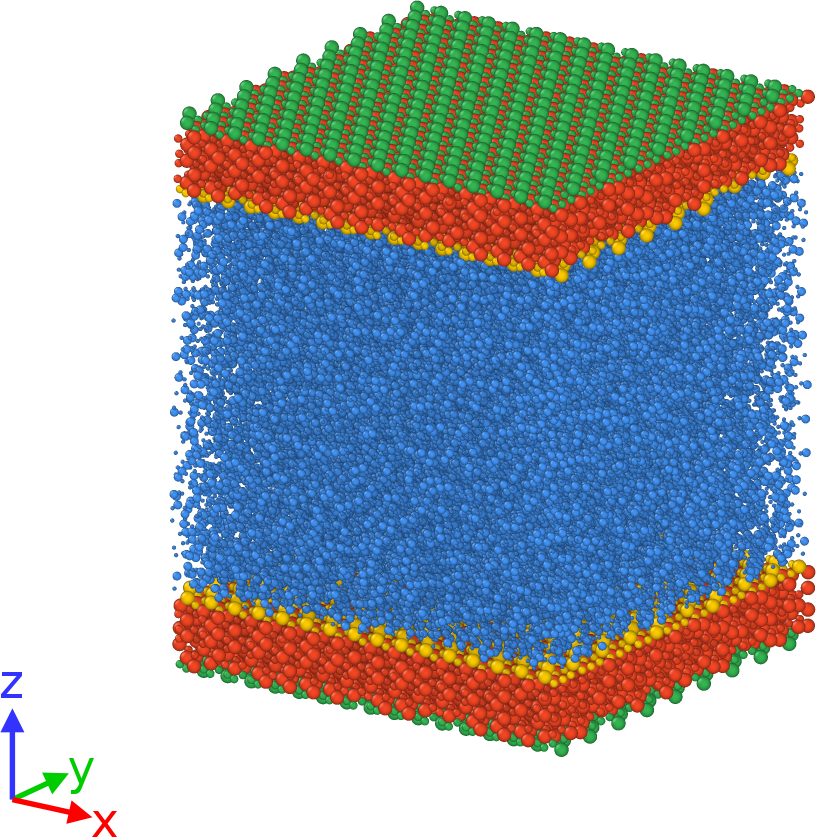
\includegraphics[width=0.25\textwidth]{DataDump/Images/5_region.png}};
			\begin{scope}[x={(fig_regions.south east)},y={(fig_regions.north west)}]
				\draw [](0,0.8) node[text width=1cm,align=center]{Top\\Wall}	;
				\draw [](0,0.53) node[]{Fluid}	;
				\draw [](0,0.27) node[text width=1cm,align=center]{Bottom\\Wall}	;

				\draw [decorate,decoration={brace}] (0.17,0.76) -- (0.17,0.86);
				\draw [decorate,decoration={brace}] (0.17,0.295) -- (0.17,0.755);
				\draw [decorate,decoration={brace}] (0.17,0.19) -- (0.17,0.29);

				\node (A) at (0.7,0.9) {} ;
				\node (B) at (1.0,1.0) [SERgreen]{Frozen} ;
				\draw [SERgreen, <- , line width=0.006*\textwidth] (A) -- (B);

				\node (C) at (0.8,0.78) {} ;
				\node (D) at (1.2,0.9) [SERorange2] {Thermostat} ;
				\draw [SERorange2, <- , line width=0.006*\textwidth] (C) -- (D);

				\node (E) at (0.8,0.74) {} ;
				\node (F) at (1.2,0.7) [SERyellow]{Free} ;
				\draw [SERyellow, <- , line width=0.006*\textwidth] (E) -- (F);
				
				\node (G) at (0.3,0.79) {} ;
				\node (H) at (0.6,0.725) []{$v/2$} ;
				\draw [ -> , line width=0.004*\textwidth] (G) -- (H);

				\node (I) at (0.3,0.23) {} ;
				\node (J) at (0.6,0.165) []{$v/2$} ;
				\draw [ <- , line width=0.004*\textwidth] (I) -- (J);

				\node (K) at (0.62,1.1) {$P$} ;
				\node (L) at (0.62,0.85) []{} ;
				\draw [ <- , line width=0.008*\textwidth] (L) -- (K);

			\end{scope}
		\end{tikzpicture}
		\caption{Structure and regions of a typical system for the simulation of confined lubricants. The system is divided in three regions, namely, the fluid, and the top and bottom walls. Within each wall, the \textit{frozen} atoms (green) are used to apply the shearing and compressive constraints, and  the \textit{thermostat} atoms (orange) to control the temperature. Both the \textit{free} (yellow) and fluid (blue) atoms are left unconstrained.}
		\label{fig:Regions}
	\end{center}
\end{figure}

For the compression and shearing stages, the temperature of the system is controlled (T = \SI{353}{\kelvin}) by a Langevin thermostat~\cite{Schneider1978} with a damping constant of \SI{0.1}{\pico\second} acting only on the middle layer of atoms in the slabs (\textit{thermostat} in Figure \ref{fig:Regions}). The thermostat was applied only in the direction perpendicular to both the sliding and compression (\emph{y}). This approach is known to be more physically meaningful than applying the thermostat directly to the confined fluid, which has been shown to significantly affect friction and flow behaviour, particularly at high shear rates~\cite{Liem1992,Bernardi2010,Yong2013}.

The compression phase is performed in two steps; first, the pressure is linearly incremented over \SI{10}{\nano\second} and then the target pressure is maintained for a further \SI{10}{\nano\second}. The density of the fluid region and the average pressure reach a steady state well within the simulation time. The different final densities are presented in Table \ref{tab:rho} which correspond to the average density of the final \SI{1}{\nano\second} of the compression phase. In agreement with the available experimental data~\cite{Griesbaum2000}, there is an increase in average density with increasing alkane chain length, as well as with increasing pressure.

\begin{table}
	\caption{Effect of confined n-alkane chain length and pressure on the average density in the fluid region (\ref{fig:Regions})}.   
	\centering     
	\begin{tabular}{c | l l  l}
		\hline\hline\\ [-2ex]

		
										&	\multicolumn{3}{c}{ $\rho \, [\SI{}{\kilogram\per\cubic\meter}]$} \\

		\hline\\ [-2ex]
		\backslashbox{Chain \\ Length}{P $[\SI{}{\giga\pascal}]$}	&	0.5		&	1.0		&	1.5	\\

		\hline\\ [-2ex]
		$C_{16}$								&	0.87	&	0.93	&	0.98	\\
		$C_{30}$							&	0.90	&	0.96	&	1.00	\\	
		$C_{60}$								&	0.91	&	0.97	&	1.01	\\	

		\hline\hline    \\[-2ex]
	\end{tabular}
	\label{tab:rho}  
\end{table}

\subsection{Shear}

After the n-alkanes are equilibrated at the target pressures (\SI{0.5}-\SI{1.5}{\giga\pascal}), the shear response of the lubricant was studied. A shear velocity gradient was imposed on the system by means of a constant velocity, $v_x = \pm v_s/2$ applied to the outermost layer of atoms in each slab (see Figure \ref{fig:Regions}) in the \emph{x} direction. The following sliding velocities were considered, $v_s$; \SI{10}{\meter\per\second}, \SI{20}{\meter\per\second}, \SI{50}{\meter\per\second} and \SI{100}{\meter\per\second}. For the simulated film thickness (approx. \SI{8}{\nano\meter}), these correspond to applied shear rates, $\dot{\gamma}$, of approximately $10^{9} - 10^{10} \text{s}^{-1}$. While these are above those encountered in real engineering components $\left(10^{6} - 10^{8} \text{s}^{-1}\right)$~\cite{Taylor2017}, lower shear rates do not reach a steady state in the available simulation time for the longer chains studied~\cite{Ewen2018}.

To verify that a nonequilibrium steady state was reached, the evolution of the mean square end-to-end distance $\left(\left< R^2 \right> \right)$, the segmental orientation $\left(\left<P_{2}^{xz} \right> \right)$~\cite{Erman1985} and the shear stress $\left(\sigma \right)$ on the surfaces in response to the fluid, were monitored. Lower sliding velocities require a longer simulation time to reach a steady state; however, they require a similar sliding distance, in agreement with experimental observations~\cite{Drummond2000}. In general, a steady state is reached in a shorter sliding distance for shorter alkanes and lower pressures. A representative case is $C_{30}$ at \SI{1.0}{\giga\pascal}, for which the evolution of $\left< R^2 \right>$, $\left<P_{2}^{xz} \right>$, and $\sigma$ are presented at four sliding velocities in Figure \ref{fig:SS}.
 
\pgfmathsetmacro{\SERFigwidth}{.035\linewidth}
\pgfmathsetmacro{\SERFigheight}{.036\linewidth}
\begin{figure}[htp]
    	\begin{center}
		\begin{gnuplot}[terminal=epslatex, terminaloptions={size \SERFigwidth cm, \SERFigheight cm color solid}]
			set multiplot layout 3,1 rowsfirst
			set format x ' '
			unset xlabel
			set key top right
			set key samplen  0.0
			set ylabel "$\\left< R^2\\right>  \\,[\\SI{}{\\square\\angstrom}]$"          
			set label at graph 0.03,0.89 left "a)"
			set lmargin at screen 0.25; set rmargin at screen 0.9
			set tmargin at screen 1.00; set bmargin at screen 0.7
			set ytics 280,40,400 
			plot [:600][260:400] 	'DataDump/Shear/C30/1.0GPa/10m_s/e2e2.plot_s'  u  (($1/1e6)*10):($2) w l  lw 3   lt 3  notitle   ,\
								'DataDump/Shear/C30/1.0GPa/20m_s/e2e2.plot_s'  u  (($1/1e6)*20):($2) w l  lw 3   lt 4  notitle   ,\
								'DataDump/Shear/C30/1.0GPa/50m_s/e2e2.plot_s'   u (($1/1e6)*50):($2) w l  lw 3   lt 5  notitle  ,\
								'DataDump/Shear/C30/1.0GPa/100m_s/e2e2.plot_s' u  (($1/1e6)*100):($2) w l  lw 3   lt 10  notitle  
			
			unset label
			set tmargin at screen 0.7; set bmargin at screen 0.4
			set ytics 0.3, 0.1, 0.6			
			set ylabel "$\\left<P_{2}^{xz}\\right>$"        
			set label at graph 0.03,0.89 left "b)"  
			plot  [:600][0.28:0.62]	'DataDump/Shear/C30/1.0GPa/10m_s/P2XZ_s.plot' u   (($1/1e6)*10):($2) w l lw 3 lt 3  notitle   ,\
								'DataDump/Shear/C30/1.0GPa/20m_s/P2XZ_s.plot' u   (($1/1e6)*20):($2) w l  lw 3  lt 4  notitle ,\
								'DataDump/Shear/C30/1.0GPa/50m_s/P2XZ_s.plot' u  (($1/1e6)*50):($2) w l  lw 3   lt 5  notitle , \
								'DataDump/Shear/C30/1.0GPa/100m_s/P2XZ_s.plot' u  (($1/1e6)*100):($2) w l  lw 3  lt 10   notitle

			unset label
			set tmargin at screen 0.4; set bmargin at screen 0.1
			set ytics 30, 30, 150 
			set ylabel "$F_L \\, [\\SI{}{\\mega\\pascal}]$" 
			set format x '%g'
			set xlabel "Distance [\\SI{}{\\nano\\meter}]"  

			set label at graph 0.03,0.89 left "c)"
			plot  [:600][60:160]	'DataDump/Shear/C30/1.0GPa/10m_s/fc_ave.dump' u (($1/1e6)*10):($2/10) w l  lw 3    lt 3    title  "\\SI{10}{\\meter\\per\\second}"   ,\
							'DataDump/Shear/C30/1.0GPa/20m_s/fc_ave.dump' u (($1/1e6)*20):($2/10) w l  lw 3    lt 4    title  "\\SI{20}{\\meter\\per\\second}"   ,\
							'DataDump/Shear/C30/1.0GPa/50m_s/fc_ave.dump' u (($1/1e6)*50):($2/10) w l  lw 3     lt 5    title  "\\SI{50}{\\meter\\per\\second}"  ,\
							'DataDump/Shear/C30/1.0GPa/100m_s/fc_ave.dump' u (($1/1e6)*100):($2/10) w l  lw 3   lt 10    title  "\\SI{100}{\\meter\\per\\second}"  

			unset multiplot
		\end{gnuplot}

		\caption{Evolution of the a) mean square end-to-end distance $\left(\left< R^2 \right>\right)$, b) the average segmental orientation  $\left(\left<P_{2}^{xz}\right>\right)$, c) the lateral (friction) force  $\left(\sigma\right)$ and d) the temperature $\left(T\right)$ for a system with alkane chains of length $C_{30}$ at a pressure of \SI{1.0}{\giga\pascal} and four  shearing velocities. The transient state begins with the application of the shear displacement of the surfaces and ends when  steady state is attained. Note that $1 \times 10^{6}$ steps correspond to \SI{1}{\nano\second}.}
		\label{fig:SS}
	\end{center}
 \end{figure}
%\FloatBarrier

Since the initial configuration is the same for all of the sliding velocities, they all have an initial value of $\left< R^2 \right> = \SI{283}{\angstrom\squared}$. After this point, $\left< R^2 \right> $ increases and then asymptotes towards a steady state value. This suggests that the chains generally unfold when shear is applied. The steady state $\left< R^2 \right>$ is lower at higher sliding velocity, as has been observed in previous simulations of similar systems at high shear rates~\cite{Cho2017}.

For ideal chains in the bulk, the average segmental orientation, $\langle P_{2}^{xz}\rangle=0.25$. This suggests a uniform distribution of the orientation of the chains, which corresponds to an average orientation angle of \SI{45}{\degree}. When under confinement, n-alkane molecules close to the surfaces tend to align parallel to them~\cite{Cho2017}, meaning that the angle between the chain and the surface is close to zero, and hence $\langle P_{2}^{xz}\rangle$ increases. In the case of $C_{30}$ at \SI{1.0}{\giga\pascal}, $\langle P_{2}^{xz}\rangle=0.32$ before shear is applied (see Figure \ref{fig:SS}b), indicating that there is a preferential orientation caused by the presence of the surfaces. When sliding is initiated, the chains begin to align with the flow direction, increasing $\langle P_{2}^{xz}\rangle$.

The shear stress was monitored through the average lateral (friction) force $F_L$ acting on the outermost layer of atoms (frozen atoms in Figure \ref{fig:Regions}) in the top and bottom slabs (divided by their area) in response to the fluid. At the onset of sliding, $F_L$ increases rapidly to reach a maximum value and then decreases before reaching a steady state, indicating stress overshoot behaviour\cite{Jeong2017}. The sliding distance needed for $F_L$ to reach a steady state is consistent with that needed for $\left< R^2 \right> $ and $\left<P_{2}^{xz} \right> $ (Figure \ref{fig:SS}).

Once the simulations reach a steady state (Figure \ref{fig:SS}), they are run for a further \SI{5}{\nano\second} to \SI{20}{\nano\second} while maintaining a constant sliding velocity and applied pressure. During the final \SI{2}{\nano\second} of the simulation, $\left< R^2 \right>$, $\left<P_{2}^{xz} \right> $, and $\sigma$ are measured and averaged. The results are presented and discussed in the next section.

%%%%%%%%%%%%%%%%%%%%%%%%%%%%%%%%%%%%%%%%%%%%%%%%%

\section{Results and Discussion}

%The effect of chain length, pressure, and shear rate on the chain extension, $\left< R^2 \right>$ and orientation, $\left<P_{2}^{xz} \right> $ are studied in Section \ref{ext}. The change in film structure and flow are investigated through mass density and velocity profiles as well as radial distribution functions in Section \ref{str}. The dependency of the friction on the chain length, pressure, and shear rate are presented in Section \ref{fri}.

\subsection{Chain extension and orientation}
\label{ext}

Longer chains will inherently have higher absolute values of $\left< R^2 \right> $, so to compare the variation of $\left< R^2 \right> $ between the different chain lengths, the mean square end-to-end distance \emph{per C-C bond}; $\left< R^2 \right>/\left(N_\text{bonds}\right)^2$ was calculated to normalize between the different chain lengths studied. The steady state $\left< R^2 \right> $ per C-C bond is presented as a function of shear rate for the different chain lengths and pressures studied in Figure \ref{fig:e2e2_v}.

 \pgfmathsetmacro{\SERFigwidth}{.035\linewidth}
\pgfmathsetmacro{\SERFigheight}{.026\linewidth}
\begin{figure}[htp]
    	\begin{center}
		\begin{gnuplot}[terminal=epslatex, terminaloptions={size \SERFigwidth cm, \SERFigheight cm color solid}]
			set key above
			set xlabel  "$\\dot{\\gamma} \\, \\left[ \\SI{}{\\per\\second} \\right]$"  
			set ylabel "$\\left< R^2 \\right>/\\left(N_\\text{bonds}\\right)^2$ [\\SI{}{\\square\\angstrom}]"
			set ytics 0.1,0.1,0.7
			set key noautotitle
			set format x  '$10^{%L}$' 
			set logscale x
			p [:2e10][0.15:0.65]	'DataDump/Shear/Compiled.plot8' i 0 u ($3/($12*1e-10)):($6/($1-1)**2):($7/($1-1)**2)  title "$\\SI{0.5}{\\giga\\pascal}$" lt 1 lc 0 ps 2,\
				'DataDump/Shear/Compiled.plot8' i 1 u ($3/($12*1e-10)):($6/($1-1)**2):($7/($1-1)**2)  title  "$\\SI{1.0}{\\giga\\pascal}$" lt 2 lc 0 ps 2,\
				'DataDump/Shear/Compiled.plot8' i 1 u ($3/($12*1e-10)):($6/($1-1)**2) w l notitle lt 2 lc 1  lw 2 ,\
				'DataDump/Shear/Compiled.plot8' i 2 u ($3/($12*1e-10)):($6/($1-1)**2):($7/($1-1)**2)  title  "$\\SI{1.5}{\\giga\\pascal}$" lt 3 lc 0 ps 2,\
				'DataDump/Shear/Compiled.plot8' i 2 u ($3/($12*1e-10)):($6/($1-1)**2) w l notitle lt 3 lc 1 lw 2 ,\
				'DataDump/Shear/Compiled.plot8' i 3 u ($3/($12*1e-10)):($6/($1-1)**2):($7/($1-1)**2)  notitle lt 1 lc 0 ps 2 ,\
				'DataDump/Shear/Compiled.plot8' i 0 u ($3/($12*1e-10)):($6/($1-1)**2) w l title "C16" lt 1 lc 1 lw 2 ,\
				'DataDump/Shear/Compiled.plot8' i 3 u ($3/($12*1e-10)):($6/($1-1)**2) w l title "C30" lt 1 lc 2 lw 2 ,\				
				'DataDump/Shear/Compiled.plot8' i 4 u ($3/($12*1e-10)):($6/($1-1)**2) w l notitle lt 2 lc 2 lw 2 ,\
				'DataDump/Shear/Compiled.plot8' i 4 u ($3/($12*1e-10)):($6/($1-1)**2):($7/($1-1)**2)  notitle lt 2 lc 0 ps 2,\
				'DataDump/Shear/Compiled.plot8' i 5 u ($3/($12*1e-10)):($6/($1-1)**2) w l notitle lt 3 lc 2 lw 2 ,\
				'DataDump/Shear/Compiled.plot8' i 5 u ($3/($12*1e-10)):($6/($1-1)**2):($7/($1-1)**2)  notitle lt 3 lc 0 ps 2 ,\
				'DataDump/Shear/Compiled.plot8' i 6 u ($3/($12*1e-10)):($6/($1-1)**2):($7/($1-1)**2)  notitle lt 1 lc 0 ps 2 ,\
				'DataDump/Shear/Compiled.plot8' i 6 u ($3/($12*1e-10)):($6/($1-1)**2) w l title 'C60' lt 1 lc 3 lw 2 ,\				
				'DataDump/Shear/Compiled.plot8' i 7 u ($3/($12*1e-10)):($6/($1-1)**2) w l notitle  lt 2 lc 3 lw 2 ,\
				'DataDump/Shear/Compiled.plot8' i 7 u ($3/($12*1e-10)):($6/($1-1)**2):($7/($1-1)**2)  notitle  lt 2 lc 0 ps 2,\
				'DataDump/Shear/Compiled.plot8' i 8 u ($3/($12*1e-10)):($6/($1-1)**2) w l notitle  lt 3 lc 3 lw 2 ,\
				'DataDump/Shear/Compiled.plot8' i 8 u ($3/($12*1e-10)):($6/($1-1)**2):($7/($1-1)**2) notitle  lt 3 lc 0 ps 2
		\end{gnuplot}
		\caption{Mean square end-to-end distance  $\left(\left< R^2 \right> \right)$ per C-C bond as a function of the shear rate $\left( \dot{\gamma} \right)$. Error bars, calculated from the standard deviation between block-averages, are omitted for clarity, but are of a similar size to the symbols.}
		\label{fig:e2e2_v}
	\end{center}
 \end{figure}

\pgfmathsetmacro{\SERFigwidth}{.035\linewidth}
\pgfmathsetmacro{\SERFigheight}{.026\linewidth}
\begin{figure}[htp]
    	\begin{center}
		\begin{gnuplot}[terminal=epslatex, terminaloptions={size \SERFigwidth cm, \SERFigheight cm color solid}]
			set key above
			set xlabel  "$\\dot{\\gamma} \\, \\left[ \\SI{}{\\per\\second} \\right]$"  
			set ylabel "$\\left<P_{2}^{xz}\\right>$"
			set key noautotitle
			set format x  '$10^{%L}$' 
			set logscale x
			p [:2e10][]	'DataDump/Shear/Compiled.plot8' i 0 u ($3/($12*1e-10)):($8) title "$\\SI{0.5}{\\giga\\pascal}$" lt 1 lc 0 ps 2,\
					'DataDump/Shear/Compiled.plot8' i 1 u ($3/($12*1e-10)):($8) title  "$\\SI{1.0}{\\giga\\pascal}$" lt 2 lc 0 ps 2,\
					'DataDump/Shear/Compiled.plot8' i 1 u ($3/($12*1e-10)):($8) w l notitle lt 2 lc 1  lw 2 ,\
					'DataDump/Shear/Compiled.plot8' i 2 u ($3/($12*1e-10)):($8) title  "$\\SI{1.5}{\\giga\\pascal}$" lt 3 lc 0 ps 2,\
					'DataDump/Shear/Compiled.plot8' i 2 u ($3/($12*1e-10)):($8) w l notitle lt 3 lc 1 lw 2 ,\
					'DataDump/Shear/Compiled.plot8' i 3 u ($3/($12*1e-10)):($8) notitle lt 1 lc 0 ps 2 ,\
					'DataDump/Shear/Compiled.plot8' i 0 u ($3/($12*1e-10)):($8) w l title "C16" lt 1 lc 1 lw 2 ,\
					'DataDump/Shear/Compiled.plot8' i 3 u ($3/($12*1e-10)):($8) w l title "C30" lt 1 lc 2 lw 2 ,\				
					'DataDump/Shear/Compiled.plot8' i 4 u ($3/($12*1e-10)):($8) w l notitle lt 2 lc 2 lw 2 ,\
					'DataDump/Shear/Compiled.plot8' i 4 u ($3/($12*1e-10)):($8) notitle lt 2 lc 0 ps 2,\
					'DataDump/Shear/Compiled.plot8' i 5 u ($3/($12*1e-10)):($8) w l notitle lt 3 lc 2 lw 2 ,\
					'DataDump/Shear/Compiled.plot8' i 5 u ($3/($12*1e-10)):($8) notitle lt 3 lc 0 ps 2 ,\
					'DataDump/Shear/Compiled.plot8' i 6 u ($3/($12*1e-10)):($8) notitle lt 1 lc 0 ps 2 ,\
					'DataDump/Shear/Compiled.plot8' i 6 u ($3/($12*1e-10)):($8) w l title 'C60' lt 1 lc 3 lw 2 ,\				
					'DataDump/Shear/Compiled.plot8' i 7 u ($3/($12*1e-10)):($8) w l notitle  lt 2 lc 3 lw 2 ,\
					'DataDump/Shear/Compiled.plot8' i 7 u ($3/($12*1e-10)):($8) notitle  lt 2 lc 0 ps 2,\
					'DataDump/Shear/Compiled.plot8' i 8 u ($3/($12*1e-10)):($8) w l notitle  lt 3 lc 3 lw 2 ,\
					'DataDump/Shear/Compiled.plot8' i 8 u ($3/($12*1e-10)):($8) notitle  lt 3 lc 0 ps 2
		\end{gnuplot}
		\caption{Average segmental orientation as a function of the shear rate $\left( \dot{\gamma} \right)$. Error bars, calculated from the standard deviation between block-averages, are omitted for clarity, but are of a similar size to the symbols.}
		\label{fig:P2_v}
	\end{center}
 \end{figure}
 
For the chain lengths and pressures studied, $\left< R^2 \right>/\left(N_\text{bonds}\right)^2$ generally decreases with increasing shear rate, suggesting less extended chain conformations. This has also been observed in previous bulk~\cite{Cui1996} and confined~\cite{Sivebaek2008,Cho2017} NEMD simulations of similar n-alkanes at high shear rates. This decrease has been attributed to strong intermolecular collisions which lead to intense chain rotation and tumbling dynamics at higher shear rates~\cite{Cho2017}. However, long chains at high pressure show the opposite trend. Longer chains are relatively less extended than shorter chains at all pressures and shear rates studied. This is the opposite trend to that observed in previous bulk NEMD simulations~\cite{Cui1996} and could thus be due to the confining walls, which constrict motion more for longer chains~\cite{Cho2017}. The chains are slightly less extended at higher pressure, although this is only discernible at low shear rates.

% CHECK
Surprisingly, there is also a general reduction of $\left<P_{2}^{xz} \right> $ with increasing shear rate (see Figure \ref{fig:P2_v}). This indicates an increase of the average angle of segments relative to the shearing direction at higher shear rate (see Appendix), meaning that the chains are less aligned with flow direction. Although such behaviour has also been observed in bulk NEMD simulations of n-alkanes at high shear rates~\cite{Padilla1992}, the opposite trend is more commonly reported~\cite{Cho2017,Cui1996}. This discrepancy can be rationalized through the high pressures applied in these simulations which lead to the fluid becoming solid-like, which is discussed further in the following section. Previous experiments~\cite{Drummond2002} and NEMD simulations~\cite{Cho2017} have shown that n-alkanes close to the confining walls align with the shear direction. Under the high pressures applied in these NEMD simulations, the ordered region extends further towards the centre of the film (Figure \ref{fig:VelProf_MDP2}), leading to a high value of $\left<P_{2}^{xz} \right> $. As the shear rate is increased, the film becomes more liquid-like (Figure \ref{fig:RDF}), and the thickness of the ordered region decreases (Figure \ref{fig:VelProf_MDP2}), and thus $\left<P_{2}^{xz} \right> $ also decreases. Consistent with previous bulk NEMD simulations~\cite{Cui1996}, longer chains tend be more aligned with the shearing direction, while the chains are slightly less aligned at higher pressure.

% Maybe have this section first
\subsection{Film structure and flow}
\label{str}

The radial distribution function (RDF), $g(r)$ for the C atoms was calculated using a cut-off distance of \SI{20}{\angstrom} (see Figure \ref{fig:RDF}). Note that atoms separated by one or two bonds were excluded from the calculations. For all of the systems and conditions studied, three intramolecular RDF peaks are found at C-C separations of: $d_1 \approx \SI{3.2}{\angstrom}$, $d_2 \approx \SI{3.9}{\angstrom}$ and $d_3 \approx \SI{5.1}{\angstrom}$ (see \ref{fig:RDF_Peaks}). The $d_1$ and $d_2$ peaks can be mostly attributed to C atoms separated by three bonds in gauche and trans conformations respectively. The latter of these is far more intense, indicating most of the chains are in extended conformations. The $d_3$ peak is mostly due to C atoms separated by four bonds, and its intensity further suggests that the chains are mostly extended conformations. This observation is consistent with the trends shown previously for $\left< R^2 \right>/\left(N_\text{bonds}\right)^2$ (Figure \ref{fig:e2e2_v}).

There are additional peaks at larger distances in Figure \ref{fig:RDF}, which are indicative of long-range order and more solid-like films. These peaks are more evident at higher pressure and lower sliding velocity, suggesting more solid-like films under these conditions. Moreover, comparing the size of the $d_1$ and $d_2$ peaks in Figure \ref{fig:RDF}, it is clear that there is a smaller trans/gauche ratio at high pressure and lower speed, a further indication of more solid-like films under these conditions~\cite{Kavitha2007}. Longer chains also appear to be more solid-like compared to shorter chains, in agreement with previous confined NEMD simulations~\cite{Sivebaek2012}.

\pgfmathsetmacro{\SERFigwidth}{.035\linewidth}
\pgfmathsetmacro{\SERFigheight}{.04\linewidth}
\begin{figure}[htp]
    	\begin{center}
		\begin{gnuplot}[terminal=epslatex, terminaloptions={size \SERFigwidth cm, \SERFigheight cm color solid}]
			set multiplot layout 4,1 rowsfirst
			set format x ' '
			unset xlabel

			set key samplen  0.0
			set label at graph 0.03,0.89 left "a) P=0.5GPa, v=10m/s"
#			set lmargin at screen 0.25; set rmargin at screen 0.9
			set tmargin at screen 1.00; set bmargin at screen 0.775
			set ylabel "g(r)"
			set key noautotitle
			set xrange [0:20]
			set yrange [0:2.5]
			set ytics 0,1,4
			plot  	'DataDump/Shear/C16/0.5GPa/10m_s_RDF/all_c_rdf_s.dump' u  ($2):($3/1.8) notitle   w l lw 2,\
		        	'DataDump/Shear/C30/0.5GPa/10m_s_RDF/all_c_rdf_s.dump' u  ($2):($3/1.8) notitle   w l lw 2,\
		        	'DataDump/Shear/C60/0.5GPa/10m_s_RDF/all_c_rdf_s.dump' u  ($2):($3/1.8) notitle   w l lw 2
	    	unset label


			set tmargin at screen 0.775; set bmargin at screen 0.550
			set label at graph 0.03,0.89 left "b) P=0.5GPa, v=100m/s"
			set ylabel "g(r)"
			set ytics 0,1,4
			set key noautotitle
			plot  	'DataDump/Shear/C16/0.5GPa/100m_s_RDF/all_c_rdf_s.dump' u  ($2):($3/1.8) notitle w l lw 2,\
		        	'DataDump/Shear/C30/0.5GPa/100m_s_RDF/all_c_rdf_s.dump' u  ($2):($3/1.8) notitle   w l lw 2,\
		        	'DataDump/Shear/C60/0.5GPa/100m_s_RDF/all_c_rdf_s.dump' u  ($2):($3/1.8) notitle  w l lw 2
	    	unset label



			set tmargin at screen 0.550; set bmargin at screen 0.325
			set label at graph 0.03,0.89 left "c) P=1.5GPa, v=10m/s"
			set ylabel "g(r)"
			set ytics 0,1,4
			set key noautotitle
			plot  	'DataDump/Shear/C16/1.5GPa/10m_s_RDF/all_c_rdf_s.dump' u  ($2):($3/1.8) notitle   w l lw 2,\
		        	'DataDump/Shear/C30/1.5GPa/10m_s_RDF/all_c_rdf_s.dump' u  ($2):($3/1.8) notitle   w l lw 2,\
		        	'DataDump/Shear/C60/1.5GPa/10m_s_RDF/all_c_rdf_s.dump' u  ($2):($3/1.8) notitle   w l lw 2
	    	unset label

			set format x '%g'
			set tmargin at screen 0.325; set bmargin at screen 0.10
			set label at graph 0.03,0.89 left "d) P=1.5GPa, v=100m/s"
			set ylabel "g(r)"
			set ytics 0,1,4
			set key noautotitle
			plot  	'DataDump/Shear/C16/1.5GPa/100m_s_RDF/all_c_rdf_s.dump' u  ($2):($3/1.8) title  'C16' w l lw 2,\
		        	'DataDump/Shear/C30/1.5GPa/100m_s_RDF/all_c_rdf_s.dump' u  ($2):($3/1.8) title  'C30' w l lw 2,\
		        	'DataDump/Shear/C60/1.5GPa/100m_s_RDF/all_c_rdf_s.dump' u  ($2):($3/1.8) title  'C60' w l lw 2
	    	unset label

			unset multiplot
		\end{gnuplot}
		\caption{Radial Distribution Function $g(r)$ (RDF) measured during the steady state of the simulations for three different chain lengths: C16, C30 and C60. a) \SI{0.5}{\giga\pascal},  \SI{10}{\meter\per\second},   b) \SI{0.5}{\giga\pascal},  \SI{100}{\meter\per\second}, c) \SI{1.5}{\giga\pascal},  \SI{10}{\meter\per\second} and    d) \SI{1.5}{\giga\pascal},  \SI{100}{\meter\per\second}.
}
		\label{fig:RDF}
	\end{center}
 \end{figure}		
%\FloatBarrier		

\begin{figure}[htp]
    	\begin{center}
		
		\begin{tikzpicture}
			\node[anchor=south west,inner sep=0] (fig_axes) at (0,0){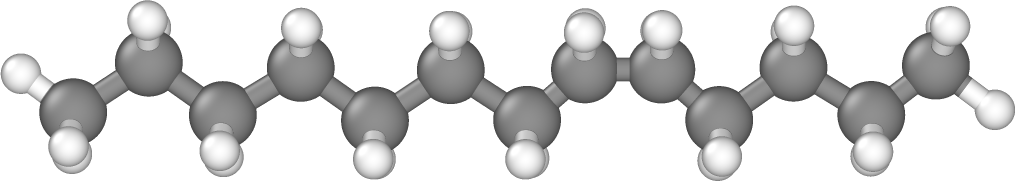
\includegraphics[width=0.8\linewidth]{DataDump/Images/RDF_Peaks.png}};
			%%%%

			\filldraw[fill=SERgray, draw=black]  	(6,2) circle (0.385*3/4) node {C};
			\filldraw[fill=SERwhite, draw=black]  	(5,2) circle (0.185) node {H};
			\draw node[] (d1_A) at (3.6,-0.5) {};
			\draw node[] (d1_B) at (4.92,-0.5) {};
			\draw node[] (d2_A) at (1.52,-0.5) {};
			\draw node[] (d3_A) at (1.4,1.99) {};
			\draw node[] (d3_B) at (2.89,1.59) {};
			\draw node[minimum width=10,minimum height=20,fill=white,rotate=53] (Cut1) at (0.069,0.85) {};
			\draw node[minimum width=10,minimum height=20,fill=white,rotate=53] (Cut2) at (6.985,0.45) {};

			\draw node[] (Cut1) at (0.0,0.5) {...};
			\draw node[] (Cut2) at (7.05,0.5) {...};

            \dimline[line style = {line width=0.7},extension start length=-0.35,extension end length=-0.35] {(d1_A)}{(d1_B)}{$d_1$};
            \dimline[line style = {line width=0.7},extension start length=-0.24,extension end length=0.0] {(d2_A)}{(d1_A)}{$d_3$};
            \dimline[line style = {line width=0.7},extension start length=0.54,extension end length=0.54] {(d3_A)}{(d3_B)}{$d_2$};

		\end{tikzpicture}

		\caption{Distances $d_1$, $d_2$ and $d_3$ between pairs of carbon atoms corresponding to the first three peaks of the radial distribution functions for all the systems. }
		\label{fig:RDF_Peaks}
	\end{center}
\end{figure}

Figure \ref{fig:VelProf_MDP2} shows the atomic mass density profile in the \emph{z}-dimension and \emph{x}-velocity profile in the \emph{z}-dimension profiles for the shortest and longest chains ($C_{16} - C_{60}$) and lowest and highest pressures ($0.5-\SI{1.5}{\giga\pascal}$) and sliding velocities ($10-\SI{100}{\meter\per\second}$) studied.

The mass density profiles in Figure \ref{fig:VelProf_MDP2} show the through-thickness layering of the fluids, which is strongest close to the walls. Generally, longer chains ($C_{60}$ in blue) show stronger layering compared to shorter chains ($C_{16}$ in purple), suggesting they form more solid-like films~\cite{Ewen2017a}. Comparing Figure \ref{fig:VelProf_MDP2}a with \ref{fig:VelProf_MDP2}b and Figure \ref{fig:VelProf_MDP2}c with \ref{fig:VelProf_MDP2}d shows that the films become less layered (particularly in the centre of the film), and thus more liquid-like at higher sliding velocity. Comparing Figure \ref{fig:VelProf_MDP2}a with \ref{fig:VelProf_MDP2}c and Figure \ref{fig:VelProf_MDP2}b with \ref{fig:VelProf_MDP2}d shows that the films become more layered and thus more solid-like at higher pressure.

The velocity profiles show deviations from planar Couette flow at the onset of shear for several of the systems and conditions studied; however, for the majority of systems and conditions (not shown), a Couette profile develops once a nonequilibrium steady state is reached (see Appendix). Figure \ref{fig:VelProf_MDP2} shows steady state velocity profiles for the systems and conditions which show deviations from planar Couette flow. At low sliding velocity and low pressure (Figure \ref{fig:VelProf_MDP2}a), the flow for $C_{16}$ (purple) remains Couette-like, whereas $C_{60}$ (blue) shows central localization (CL). CL describes the outer solid-like regions of the fluid moving at the same velocity as the proximal walls with only the centre of the film being sheared~\cite{Heyes2012}. The transition from Couette flow to CL has been observed for viscous polymers using in-contact photoluminescence experiments under EHL conditions~\cite{Galmiche2016}. It has also been observed in previous NEMD simulations of atomic fluids~\cite{Heyes2012,Gattinoni2013,Mackowiak2016} as well as alkanes and traction fluids~\cite{Ewen2017a} under EHL conditions. At low sliding velocity and high pressure, (Figure \ref{fig:VelProf_MDP2}c), $C_{16}$ again shows Couette flow while $C_{60}$ shows plug slip (PS). Here, the central part of the film becomes solid-like and shear is localized near (but not at) the fluid-wall interface~\cite{Heyes2012}. The transition from Couette flow to PS has been observed for viscous polymers using in-contact photoluminescence experiments under EHL conditions~\cite{Ponjavic2014a}. The transition from CL to PS with increasing pressure has been observed in previous NEMD simulations of atomic fluids~\cite{Heyes2012,Gattinoni2013,Mackowiak2016} and traction fluids~\cite{Ewen2017a}. At high sliding velocity, linear velocity profiles are recovered due to melting of the solid-like regions. At high sliding velocity and low pressure (Figure \ref{fig:VelProf_MDP2}b), a small amount of boundary slip at the fluid-wall interface (slip length < 1 nm) is observed for both $C_{16}$ and $C_{60}$, in agreement with previous NEMD simulations of thinner films~\cite{Sivebaek2010,Ta2017}. The slip length increases with increasing pressure (Figure \ref{fig:VelProf_MDP2}d) as has been observed in previous NEMD simulations~\cite{Ta2017} and in-contact photoluminescence experiments~\cite{Ponjavic2014}.
%-1.39716 , 81.0918
%-1.39716 , 81.0918
%-1.51672, 75.8545
%-1.51672, 75.8545

%-1.34156, 81.2584
%-1.34156, 81.2584



%-1.47486, 72.8981
%-1.47486, 72.8981
%-1.5611, 70.1875
%-1.5611, 70.1875

%-1.55172, 74.2276
%-1.55172, 74.2276
%-1.5611, 70.1875
%-1.5611, 70.1875

\pgfmathsetmacro{\SERFigwidth}{.035\linewidth}
\pgfmathsetmacro{\SERFigheight}{.02\linewidth}
\begin{figure}[htp]
    	\begin{center}
		\begin{gnuplot}[terminal=epslatex, terminaloptions={size \SERFigwidth cm, \SERFigheight cm color solid}]
			binwidth=2
			binwidth2=4
			bin(x,width)=width*floor(x/width)
			set format y2 '%g'
			set label at graph 0.03,0.89 left "a)"
			set ylabel "x Velocity $\\left[ \\SI{}{\\meter\\per\\second} \\right]$"
			set y2label "AMD $\\left[ \\SI{}{\\gram\\per\\cubic\\centi\\meter} \\right]$ "
			set key noautotitle
			set xrange [-50:50]
			set y2range [0:3]
			set ytics  -5,2.5,5
			set ytics nomirror
			set y2tics 0,1,4
			set xlabel "z coordinate"  
			plot  	[][-6:6]  'DataDump/Shear/C16/0.5GPa/10m_s/fluid_mdp_z_s.dump' u ($2-39.84732):($4) w l  lt 1 axes x1y2,\    								
				              'DataDump/Shear/C16/0.5GPa/10m_s/vel_prof_x_s.dump'  u (bin($2-39.84732,binwidth2)):($4*100) smooth unique lt 1 dashtype 4 lw 5,\	
                             		     'DataDump/Shear/C60/0.5GPa/10m_s/fluid_mdp_z_s.dump' u ($2-37.16889):($4) w l  lt 3  axes x1y2,\ 								
				              'DataDump/Shear/C60/0.5GPa/10m_s/vel_prof_x_s.dump'  u (bin($2-37.16889,binwidth)):($4*100) smooth unique lt 3 dashtype 4 lw 5	
		\end{gnuplot}
		\begin{gnuplot}[terminal=epslatex, terminaloptions={size \SERFigwidth cm, \SERFigheight cm color solid}]
			binwidth=2
			bin(x,width)=width*floor(x/width)
			set format y2 '%g'
			set label at graph 0.03,0.89 left "b)"
			set ylabel "x Velocity $\\left[ \\SI{}{\\meter\\per\\second} \\right]$"
			set y2label "AMD $\\left[ \\SI{}{\\gram\\per\\cubic\\centi\\meter} \\right]$ "
			set key noautotitle
			set xrange [-50:50]
			set y2range [0:3]
			set ytics  -50,25,50
			set ytics nomirror
			set y2tics 0,1,4
			set xlabel "z coordinate"  
			plot  	[][-60:60]  'DataDump/Shear/C16/0.5GPa/100m_s/fluid_mdp_z_s.dump' u ($2-41):($4) w l  lt 1 axes x1y2,\ 								
				              'DataDump/Shear/C16/0.5GPa/100m_s/vel_prof_x_s.dump'  u (bin($2-41,binwidth)):($4*100) smooth unique lt 1 dashtype 4  lw 5,\ 	
                             		    'DataDump/Shear/C60/0.5GPa/100m_s/fluid_mdp_z_s.dump' u ($2-39.11):($4) w l  lt 3  axes x1y2,\
				              'DataDump/Shear/C60/0.5GPa/100m_s/vel_prof_x_s.dump'  u (bin($2-39.11,binwidth)):($4*100) smooth unique lt 3 dashtype 4  lw 5
		\end{gnuplot}
		\begin{gnuplot}[terminal=epslatex, terminaloptions={size \SERFigwidth cm, \SERFigheight cm color solid}]
			binwidth=4
			binwidth2=3
			bin(x,width)=width*floor(x/width)
			set format y2 '%g'
			set label at graph 0.03,0.89 left "c)"
			set ylabel "x Velocity $\\left[ \\SI{}{\\meter\\per\\second} \\right]$"
			set y2label "AMD $\\left[ \\SI{}{\\gram\\per\\cubic\\centi\\meter} \\right]$ "
			set key noautotitle
			set xrange [-50:50]
			set y2range [0:3]
			set ytics  -5,2.5,5
			set ytics nomirror
			set y2tics 0,1,4
			set xlabel "z coordinate"  
			plot  	[][-6:6]  'DataDump/Shear/C16/1.5GPa/10m_s/fluid_mdp_z_s.dump' u ($2-35.7116):($4) w l  lt 1 axes x1y2,\ 								
				              'DataDump/Shear/C16/1.5GPa/10m_s/vel_prof_x_s.dump'  u (bin($2-35.7116,binwidth2)):($4*100) smooth unique lt 1 dashtype 4  lw 5,\	
                             		    'DataDump/Shear/C60/1.5GPa/10m_s/fluid_mdp_z_s.dump' u ($2-34.3132):($4) w l  lt 3  axes x1y2,\ 								
				              'DataDump/Shear/C60/1.5GPa/10m_s/vel_prof_x_s.dump'  u (bin($2-34.3132,binwidth)):($4*100) smooth unique lt 3 dashtype 4  lw 5		
		\end{gnuplot}
		\begin{gnuplot}[terminal=epslatex, terminaloptions={size \SERFigwidth cm, \SERFigheight cm color solid}]
		set key top center
			binwidth=2
			bin(x,width)=width*floor(x/width)
			set format y2 '%g'
			set label at graph 0.03,0.89 left "d)"
			set ylabel "x Velocity $\\left[ \\SI{}{\\meter\\per\\second} \\right]$"
			set y2label "AMD $\\left[ \\SI{}{\\gram\\per\\cubic\\centi\\meter} \\right]$ "
			set key noautotitle
			set xrange [-50:50]
			set y2range [0:3]
			set ytics  -50,25,50
			set ytics nomirror
			set y2tics 0,1,4
			set xlabel "z coordinate"  
			plot  	[][-60:60]  'DataDump/Shear/C16/1.5GPa/100m_s/fluid_mdp_z_s.dump' u ($2-36.3379):($4) w l  lt 1 axes x1y2 title "C16",\ 						
				              'DataDump/Shear/C16/1.5GPa/100m_s/vel_prof_x_s.dump'  u (bin($2-36.3379,binwidth)):($4*100) smooth unique lt 1 dashtype 4  lw 5,\ 
                             		     'DataDump/Shear/C60/1.5GPa/100m_s/fluid_mdp_z_s.dump' u ($2-34.8132):($4) w l  lt 3  axes x1y2 title "C60",\ 						
				              'DataDump/Shear/C60/1.5GPa/100m_s/vel_prof_x_s.dump'  u (bin($2-34.8132,binwidth)):($4*100) smooth unique lt 3 dashtype 4  lw 5 	
		\end{gnuplot}
		
		\caption{Velocity (solid lines) and mass density (dotted lines) measured during the steady state of the simulations for two different chain lenghts: C16 and C60. a) \SI{0.5}{\giga\pascal},  \SI{10}{\meter\per\second},   b) \SI{0.5}{\giga\pascal},  \SI{100}{\meter\per\second}, c) \SI{1.5}{\giga\pascal},  \SI{10}{\meter\per\second} and    d) \SI{1.5}{\giga\pascal},  \SI{100}{\meter\per\second}} 
		\label{fig:VelProf_MDP2}
	\end{center}
 \end{figure}

\subsection{Friction}
\label{fri}

Figure \ref{fig:FL_FN} shows that shear stress increases linearly with increasing pressure. For all of the the systems and conditions studied, there is an approximately zero intercept in Figure \ref{fig:FL_FN}. This suggests that it appropriate to calculate the friction coefficient, $\mu$, using the Amontons–Coulomb law under the high load approximation; $F_L/F_N = F_0/F_N + \mu \approx \mu$, where $F_L$ and $F_N$ are respectively the mean lateral force (or shear stress) and normal force acting on the outer layer of atoms in each slab in response to the fluid, and $F_0$ is the load-independent Derjaguin offset representing adhesive surface forces~\cite{Ewen2017a}.

\pgfmathsetmacro{\SERFigwidth}{.035\linewidth}
\pgfmathsetmacro{\SERFigheight}{.026\linewidth}
\begin{figure}[htp]
    	\begin{center}
		\begin{gnuplot}[terminal=epslatex, terminaloptions={size \SERFigwidth cm, \SERFigheight cm color solid}]
			set key above
			set xlabel "$F_N \\, [\\SI{}{\\mega\\pascal}]$"
			set ylabel "$F_L \\, [\\SI{}{\\mega\\pascal}]$"
			set ytics 0,20,120
			set key noautotitle
            p [400:1600][]	'DataDump/Shear/Compiled_p.plot8' i 0 u ($2*1000):($4/10) w p title "$\\SI{10}{\\meter\\per\\second}$" lt 1 lc 0 ps 2,\
                'DataDump/Shear/Compiled_p.plot8' i 1 u ($2*1000):($4/10) w p title "$\\SI{20}{\\meter\\per\\second}$" lt 2 lc 0 ps 2,\
	    		'DataDump/Shear/Compiled_p.plot8' i 1 u ($2*1000):($4/10) w l notitle  lt 1 lc 1 lw 2	,\
                'DataDump/Shear/Compiled_p.plot8' i 2 u ($2*1000):($4/10) w p title "$\\SI{50}{\\meter\\per\\second}$" lt 3 lc 0 ps 2,\
	    		'DataDump/Shear/Compiled_p.plot8' i 2 u ($2*1000):($4/10) w l notitle  lt 1 lc 1 lw 2	,\
                'DataDump/Shear/Compiled_p.plot8' i 3 u ($2*1000):($4/10) w p title "$\\SI{100}{\\meter\\per\\second}$" lt 4 lc 0 ps 2,\
	    		'DataDump/Shear/Compiled_p.plot8' i 3 u ($2*1000):($4/10) w l notitle  lt 1 lc 1 lw 2 ,\
                'DataDump/Shear/Compiled_p.plot8' i 4 u ($2*1000):($4/10) w p notitle  lt 1 lc 0 ps 2,\
	    		'DataDump/Shear/Compiled_p.plot8' i 0 u ($2*1000):($4/10) w l title "C16" lt 1 lc 1 lw 2 ,\
	    		'DataDump/Shear/Compiled_p.plot8' i 4 u ($2*1000):($4/10) w l title "C30" lt 1 lc 2 lw 2 ,\	    		
                'DataDump/Shear/Compiled_p.plot8' i 5 u ($2*1000):($4/10) w p notitle lt 2 lc 0 ps 2,\
	    		'DataDump/Shear/Compiled_p.plot8' i 5 u ($2*1000):($4/10) w l notitle lt 1 lc 2 lw 2 ,\
	            'DataDump/Shear/Compiled_p.plot8' i 6 u ($2*1000):($4/10) w p notitle lt 3 lc 0 ps 2,\
	    		'DataDump/Shear/Compiled_p.plot8' i 6 u ($2*1000):($4/10) w l notitle lt 1 lc 2 lw 2 ,\	    		
                'DataDump/Shear/Compiled_p.plot8' i 7 u ($2*1000):($4/10) w p notitle lt 4 lc 0 ps 2,\
	    		'DataDump/Shear/Compiled_p.plot8' i 7 u ($2*1000):($4/10) w l notitle lt 1 lc 2 lw 2 ,\	    		
                'DataDump/Shear/Compiled_p.plot8' i 8 u ($2*1000):($4/10) w p notitle  lt 1 lc 0 ps 2,\
	    		'DataDump/Shear/Compiled_p.plot8' i 8 u ($2*1000):($4/10) w l title "C60" lt 1 lc 3 lw 2 ,\	    		
                'DataDump/Shear/Compiled_p.plot8' i 9 u ($2*1000):($4/10) w p notitle lt 2 lc 0 ps 2,\
	    		'DataDump/Shear/Compiled_p.plot8' i 9 u ($2*1000):($4/10) w l notitle lt 1 lc 3 lw 2 ,\
	            'DataDump/Shear/Compiled_p.plot8' i 10 u ($2*1000):($4/10) w p notitle lt 3 lc 0 ps 2,\
	    		'DataDump/Shear/Compiled_p.plot8' i 10 u ($2*1000):($4/10) w l notitle lt 1 lc 3 lw 2 ,\	    		
                'DataDump/Shear/Compiled_p.plot8' i 11 u ($2*1000):($4/10) w p notitle lt 4 lc 0 ps 2,\
	    		'DataDump/Shear/Compiled_p.plot8' i 11 u ($2*1000):($4/10) w l notitle lt 1 lc 3 lw 2 	    		
	    		\end{gnuplot}
		\caption{Lateral (friction) force, $F_L$, as a function of the applied pressure, $F_N$, on the outer layer of atoms in the top and bottom slabs measured after reaching steady stat}
		\label{fig:FL_FN}
	\end{center}
 \end{figure}
%\FloatBarrier

% \pgfmathsetmacro{\SERFigwidth}{.035\linewidth}
% \pgfmathsetmacro{\SERFigheight}{.026\linewidth}
% \begin{figure}[htp]
%     	\begin{center}
% 		\begin{gnuplot}[terminal=pdf, terminaloptions={size \SERFigwidth cm, \SERFigheight cm color solid}]
% 			set key above
% 			set xlabel  "x Velocity $\\left[ \\SI{}{\\meter\\per\\second} \\right]$"  
% 			set ylabel "$F_L \\, [\\SI{}{\\mega\\pascal}]$"
% 			set ytics 20,20,120
% 			set key noautotitle
% 			p [:110][15:125]	'Data/Shear/Compiled_e2e2_v.plot8.plot' i 0 u ($3):($4/10):($5/10) w p title "$\\SI{0.5}{\\giga\\pascal}$" lt 1 lc 0 ps 1,\
% 				'Data/Shear/Compiled_e2e2_v.plot8.plot' i 1 u ($3):($4/10):($5/10) w p title  "$\\SI{1.0}{\\giga\\pascal}$" lt 2 lc 0 ps 1,\
% 				'Data/Shear/Compiled_e2e2_v.plot8.plot' i 1 u ($3):($4/10) w l notitle lt 2 lc 1  lw 2 ,\
% 				'Data/Shear/Compiled_e2e2_v.plot8.plot' i 2 u ($3):($4/10):($5/10) w p title  "$\\SI{1.5}{\\giga\\pascal}$" lt 3 lc 0 ps 1,\
% 				'Data/Shear/Compiled_e2e2_v.plot8.plot' i 2 u ($3):($4/10) w l notitle lt 3 lc 1 lw 2 ,\
% 				'Data/Shear/Compiled_e2e2_v.plot8.plot' i 3 u ($3):($4/10):($5/10) w p notitle lt 1 lc 0 ps 1 ,\
% 				'Data/Shear/Compiled_e2e2_v.plot8.plot' i 0 u ($3):($4/10) w l title "C16" lt 1 lc 1 lw 2 ,\
% 				'Data/Shear/Compiled_e2e2_v.plot8.plot' i 3 u ($3):($4/10) w l title "C30" lt 1 lc 2 lw 2 ,\				
% 				'Data/Shear/Compiled_e2e2_v.plot8.plot' i 4 u ($3):($4/10) w l notitle lt 2 lc 2 lw 2 ,\
% 				'Data/Shear/Compiled_e2e2_v.plot8.plot' i 4 u ($3):($4/10):($5/10) w p notitle lt 2 lc 0 ps 1,\
% 				'Data/Shear/Compiled_e2e2_v.plot8.plot' i 5 u ($3):($4/10) w l notitle lt 3 lc 2 lw 2 ,\
% 				'Data/Shear/Compiled_e2e2_v.plot8.plot' i 5 u ($3):($4/10):($5/10) w p notitle lt 3 lc 0 ps 1 ,\
% 				'Data/Shear/Compiled_e2e2_v.plot8.plot' i 6 u ($3):($4/10):($5/10) w p notitle lt 1 lc 0 ps 1 ,\
% 				'Data/Shear/Compiled_e2e2_v.plot8.plot' i 6 u ($3):($4/10) w l title 'C60' lt 1 lc 3 lw 2 ,\				
% 				'Data/Shear/Compiled_e2e2_v.plot8.plot' i 7 u ($3):($4/10) w l notitle  lt 2 lc 3 lw 2 ,\
% 				'Data/Shear/Compiled_e2e2_v.plot8.plot' i 7 u ($3):($4/10):($5/10) w p notitle  lt 2 lc 0 ps 1,\
% 				'Data/Shear/Compiled_e2e2_v.plot8.plot' i 8 u ($3):($4/10) w l notitle  lt 3 lc 3 lw 2 ,\
% 				'Data/Shear/Compiled_e2e2_v.plot8.plot' i 8 u ($3):($4/10):($5/10) w p notitle  lt 3 lc 0 ps 1,\
% 		\end{gnuplot}
% 		\caption{Lateral (friction) force as a function of the shearing velocity measured after reaching steady state. Error bars, calculated from the standard deviation between the trajectory time-averages, are omitted for clarity, but are of a similar size to the symbols.}
% 		\label{fig:FL_v1}
% 	\end{center}
%  \end{figure}

\pgfmathsetmacro{\SERFigwidth}{.035\linewidth}
\pgfmathsetmacro{\SERFigheight}{.026\linewidth}
\begin{figure}[htp]
    	\begin{center}
		\begin{gnuplot}[terminal=epslatex, terminaloptions={size \SERFigwidth cm, \SERFigheight cm color solid}]
			set key above
			set ylabel "$F_L \\, [\\SI{}{\\mega\\pascal}]$"
			set ytics 0,20,150
			set key noautotitle
			set xlabel  "$\\dot{\\gamma} \\, \\left[ \\SI{}{\\per\\second} \\right]$"  
			set format x  '$10^{%L}$' 
			set logscale x
			p [:2e10][0:150]	'DataDump/Shear/Compiled.plot8' i 0 u ($3/($12*1e-10)):($4/10):($5/10) w p title "$\\SI{0.5}{\\giga\\pascal}$" lt 1 lc 0 ps 2,\
				'DataDump/Shear/Compiled.plot8' i 1 u ($3/($12*1e-10)):($4/10):($5/10) w p title  "$\\SI{1.0}{\\giga\\pascal}$" lt 2 lc 0 ps 2,\
				'DataDump/Shear/Compiled.plot8' i 1 u ($3/($12*1e-10)):($4/10) w l notitle lt 2 lc 1  lw 2 ,\
				'DataDump/Shear/Compiled.plot8' i 2 u ($3/($12*1e-10)):($4/10):($5/10) w p title  "$\\SI{1.5}{\\giga\\pascal}$" lt 3 lc 0 ps 2,\
				'DataDump/Shear/Compiled.plot8' i 2 u ($3/($12*1e-10)):($4/10) w l notitle lt 3 lc 1 lw 2 ,\
				'DataDump/Shear/Compiled.plot8' i 3 u ($3/($12*1e-10)):($4/10):($5/10) w p notitle lt 1 lc 0 ps 2 ,\
				'DataDump/Shear/Compiled.plot8' i 0 u ($3/($12*1e-10)):($4/10) w l title "C16" lt 1 lc 1 lw 2 ,\
				'DataDump/Shear/Compiled.plot8' i 3 u ($3/($12*1e-10)):($4/10) w l title "C30" lt 1 lc 2 lw 2 ,\				
				'DataDump/Shear/Compiled.plot8' i 4 u ($3/($12*1e-10)):($4/10) w l notitle lt 2 lc 2 lw 2 ,\
				'DataDump/Shear/Compiled.plot8' i 4 u ($3/($12*1e-10)):($4/10):($5/10) w p notitle lt 2 lc 0 ps 2,\
				'DataDump/Shear/Compiled.plot8' i 5 u ($3/($12*1e-10)):($4/10) w l notitle lt 3 lc 2 lw 2 ,\
				'DataDump/Shear/Compiled.plot8' i 5 u ($3/($12*1e-10)):($4/10):($5/10) w p notitle lt 3 lc 0 ps 2 ,\
				'DataDump/Shear/Compiled.plot8' i 6 u ($3/($12*1e-10)):($4/10):($5/10) w p notitle lt 1 lc 0 ps 2 ,\
				'DataDump/Shear/Compiled.plot8' i 6 u ($3/($12*1e-10)):($4/10) w l title 'C60' lt 1 lc 3 lw 2 ,\				
				'DataDump/Shear/Compiled.plot8' i 7 u ($3/($12*1e-10)):($4/10) w l notitle  lt 2 lc 3 lw 2 ,\
				'DataDump/Shear/Compiled.plot8' i 7 u ($3/($12*1e-10)):($4/10):($5/10) w p notitle  lt 2 lc 0 ps 2,\
				'DataDump/Shear/Compiled.plot8' i 8 u ($3/($12*1e-10)):($4/10) w l notitle  lt 3 lc 3 lw 2 ,\
				'DataDump/Shear/Compiled.plot8' i 8 u ($3/($12*1e-10)):($4/10):($5/10) w p notitle  lt 3 lc 0 ps 2,\
		\end{gnuplot}
		\caption{Shear stress as a function of the shear rate $\left( \dot{\gamma} \right)$ measured after reaching steady state. Error bars, calculated from the standard deviation between the trajectory time-averages, are omitted for clarity, but are of a similar size to the symbols.}
		\label{fig:FL_v1a}
	\end{center}
 \end{figure}

% \pgfmathsetmacro{\SERFigwidth}{.035\linewidth}
% \pgfmathsetmacro{\SERFigheight}{.026\linewidth}
% \begin{figure}[htp]
%     	\begin{center}
% 		\begin{gnuplot}[terminal=pdf, terminaloptions={size \SERFigwidth cm, \SERFigheight cm color solid}]
% 			set key above
% 			set xlabel  "x Velocity $\\left[ \\SI{}{\\meter\\per\\second} \\right]$"  
% 			set ytics 0.04,0.01,0.08
% 			set ylabel "$\\mu$"
% 			set key noautotitle
% 			p [:110][0.038:0.082]	'Data/Shear/Compiled_e2e2_v.plot8.plot' i 0 u ($3):(($4/10)/($2*1000)) w p title "$\\SI{0.5}{\\giga\\pascal}$" lt 1 lc 0 ps 1,\
% 			        	'Data/Shear/Compiled_e2e2_v.plot8.plot' i 1 u ($3):(($4/10)/($2*1000)) w p title  "$\\SI{1.0}{\\giga\\pascal}$" lt 2 lc 0 ps 1,\
% 			        	'Data/Shear/Compiled_e2e2_v.plot8.plot' i 1 u ($3):(($4/10)/($2*1000)) w l notitle lt 2 lc 1  lw 2 ,\
% 			        	'Data/Shear/Compiled_e2e2_v.plot8.plot' i 2 u ($3):(($4/10)/($2*1000)) w p title  "$\\SI{1.5}{\\giga\\pascal}$" lt 3 lc 0 ps 1,\
% 			        	'Data/Shear/Compiled_e2e2_v.plot8.plot' i 2 u ($3):(($4/10)/($2*1000)) w l notitle lt 3 lc 1 lw 2 ,\
% 			        	'Data/Shear/Compiled_e2e2_v.plot8.plot' i 3 u ($3):(($4/10)/($2*1000)) w p notitle lt 1 lc 0 ps 1 ,\
%         				'Data/Shear/Compiled_e2e2_v.plot8.plot' i 0 u ($3):(($4/10)/($2*1000)) w l title "C16" lt 1 lc 1 lw 2 ,\
% 		        		'Data/Shear/Compiled_e2e2_v.plot8.plot' i 3 u ($3):(($4/10)/($2*1000)) w l title "C30" lt 1 lc 2 lw 2 ,\				
% 				        'Data/Shear/Compiled_e2e2_v.plot8.plot' i 4 u ($3):(($4/10)/($2*1000)) w l notitle lt 2 lc 2 lw 2 ,\
% 				        'Data/Shear/Compiled_e2e2_v.plot8.plot' i 4 u ($3):(($4/10)/($2*1000)) w p notitle lt 2 lc 0 ps 1,\
%         				'Data/Shear/Compiled_e2e2_v.plot8.plot' i 5 u ($3):(($4/10)/($2*1000)) w l notitle lt 3 lc 2 lw 2 ,\
% 		        		'Data/Shear/Compiled_e2e2_v.plot8.plot' i 5 u ($3):(($4/10)/($2*1000)) w p notitle lt 3 lc 0 ps 1 ,\
% 				        'Data/Shear/Compiled_e2e2_v.plot8.plot' i 6 u ($3):(($4/10)/($2*1000)) w p notitle lt 1 lc 0 ps 1 ,\
%         				'Data/Shear/Compiled_e2e2_v.plot8.plot' i 6 u ($3):(($4/10)/($2*1000)) w l title 'C60' lt 1 lc 3 lw 2 ,\				
% 		        		'Data/Shear/Compiled_e2e2_v.plot8.plot' i 7 u ($3):(($4/10)/($2*1000)) w l notitle  lt 2 lc 3 lw 2 ,\
% 				        'Data/Shear/Compiled_e2e2_v.plot8.plot' i 7 u ($3):(($4/10)/($2*1000)) w p notitle  lt 2 lc 0 ps 1,\
%         	   			'Data/Shear/Compiled_e2e2_v.plot8.plot' i 8 u ($3):(($4/10)/($2*1000)) w l notitle  lt 3 lc 3 lw 2 ,\
% 			        	'Data/Shear/Compiled_e2e2_v.plot8.plot' i 8 u ($3):(($4/10)/($2*1000)) w p notitle  lt 3 lc 0 ps 1,\
% 		\end{gnuplot}
% 		\caption{Friction coefficient $\mu$ as a function of the shearing velocity measured after reaching steady state.}
% 		\label{fig:FL_v}
% 	\end{center}
%  \end{figure}

\pgfmathsetmacro{\SERFigwidth}{.035\linewidth}
\pgfmathsetmacro{\SERFigheight}{.026\linewidth}
\begin{figure}[htp]
    	\begin{center}
		\begin{gnuplot}[terminal=epslatex, terminaloptions={size \SERFigwidth cm, \SERFigheight cm color solid}]
			set key above
			set ylabel "$\\mu$"
			set key noautotitle
			set ytics 0.04,0.01,0.2
			set xlabel  "$\\dot{\\gamma} \\, \\left[ \\SI{}{\\per\\second} \\right]$"  
			set format x  '$10^{%L}$' 
			set logscale x
			p [:2e10][0.04:0.13]	'DataDump/Shear/Compiled.plot8' i 0 u ($3/($12*1e-10)):(($4/10)/($2*1000)) w p title "$\\SI{0.5}{\\giga\\pascal}$" lt 1 lc 0 ps 2,\
			        	'DataDump/Shear/Compiled.plot8' i 1 u ($3/($12*1e-10)):(($4/10)/($2*1000)) w p title  "$\\SI{1.0}{\\giga\\pascal}$" lt 2 lc 0 ps 2,\
			        	'DataDump/Shear/Compiled.plot8' i 1 u ($3/($12*1e-10)):(($4/10)/($2*1000)) w l notitle lt 2 lc 1  lw 2 ,\
			        	'DataDump/Shear/Compiled.plot8' i 2 u ($3/($12*1e-10)):(($4/10)/($2*1000)) w p title  "$\\SI{1.5}{\\giga\\pascal}$" lt 3 lc 0 ps 2,\
			        	'DataDump/Shear/Compiled.plot8' i 2 u ($3/($12*1e-10)):(($4/10)/($2*1000)) w l notitle lt 3 lc 1 lw 2 ,\
			        	'DataDump/Shear/Compiled.plot8' i 3 u ($3/($12*1e-10)):(($4/10)/($2*1000)) w p notitle lt 1 lc 0 ps 2 ,\
        				'DataDump/Shear/Compiled.plot8' i 0 u ($3/($12*1e-10)):(($4/10)/($2*1000)) w l title "C16" lt 1 lc 1 lw 2 ,\
		        		'DataDump/Shear/Compiled.plot8' i 3 u ($3/($12*1e-10)):(($4/10)/($2*1000)) w l title "C30" lt 1 lc 2 lw 2 ,\				
				        'DataDump/Shear/Compiled.plot8' i 4 u ($3/($12*1e-10)):(($4/10)/($2*1000)) w l notitle lt 2 lc 2 lw 2 ,\
				        'DataDump/Shear/Compiled.plot8' i 4 u ($3/($12*1e-10)):(($4/10)/($2*1000)) w p notitle lt 2 lc 0 ps 2,\
        				'DataDump/Shear/Compiled.plot8' i 5 u ($3/($12*1e-10)):(($4/10)/($2*1000)) w l notitle lt 3 lc 2 lw 2 ,\
		        		'DataDump/Shear/Compiled.plot8' i 5 u ($3/($12*1e-10)):(($4/10)/($2*1000)) w p notitle lt 3 lc 0 ps 2 ,\
				        'DataDump/Shear/Compiled.plot8' i 6 u ($3/($12*1e-10)):(($4/10)/($2*1000)) w p notitle lt 1 lc 0 ps 2 ,\
        				'DataDump/Shear/Compiled.plot8' i 6 u ($3/($12*1e-10)):(($4/10)/($2*1000)) w l title 'C60' lt 1 lc 3 lw 2 ,\				
		        		'DataDump/Shear/Compiled.plot8' i 7 u ($3/($12*1e-10)):(($4/10)/($2*1000)) w l notitle  lt 2 lc 3 lw 2 ,\
				        'DataDump/Shear/Compiled.plot8' i 7 u ($3/($12*1e-10)):(($4/10)/($2*1000)) w p notitle  lt 2 lc 0 ps 2,\
        	   			'DataDump/Shear/Compiled.plot8' i 8 u ($3/($12*1e-10)):(($4/10)/($2*1000)) w l notitle  lt 3 lc 3 lw 2 ,\
			        	'DataDump/Shear/Compiled.plot8' i 8 u ($3/($12*1e-10)):(($4/10)/($2*1000)) w p notitle  lt 3 lc 0 ps 2,\
		\end{gnuplot}
		\caption{Friction coefficient $\mu$ as a function of the shear rate $\left( \dot{\gamma} \right)$ measured after reaching steady state.}
		\label{fig:FL_va}
	\end{center}
 \end{figure}
 
Figure \ref{fig:FL_v1a} shows the change in the shear stress, $\sigma$, with logarithmic sliding velocity and Figure \ref{fig:FL_va} shows the same data as a friction coefficient, $\mu$. In the ranges studied, $\sigma$ is more sensitive to the pressure than the chain length, particularly at high shear rates. In general, longer chains give higher $\sigma$ than shorter chains, as expected due to their higher bulk viscosity~\cite{Zhang2017}. This trend has also been observed in previous NEMD simulations of thinner films at lower pressure~\cite{Koike1998,Sivebaek2008,Sivebaek2010,Savio2012}. The difference in $\sigma$ between chain lengths decreases with increasing shear rate, such that they are almost identical at the highest shear rate studied ($\approx \SI{e10}{\per\second}$). Tribology experiments~\cite{Ewen2017a, Zhang2017} and engineering components~\cite{Taylor2017} operate at lower shear rates than those accessible through NEMD simulations~\cite{Ewen2018}. A larger increase in $\sigma$ with increasing chain length can be expected under these lower shear rates than was observed here.

At low pressure, $\sigma$ increases linearly with the logarithmic shear rate, as is commonly observed for lubricants in macroscopic EHL friction experiments~\cite{Ewen2017a}. Such behaviour has also been observed in previous NEMD simulations of linear $C_{20}$ confined (6 molecular layers) between polymer-like surfaces at low pressure (\SI{10}{\mega\pascal})~\cite{Sivebaek2010}. At intermediate pressure, the  $\sigma$ is relatively independent of the velocity, in line with Coulomb's law for dry friction. The transition to this behaviour, above the limiting shear stress, has been observed for several model lubricants in macroscopic friction experiments~\cite{Martinie2016a}. Similar behaviour has also been observed in previous NEMD simulations of linear $C_{60}$ confined (6 molecular layers) between polymer-like surfaces at low pressure (\SI{10}{\mega\pascal})~\cite{Sivebaek2010}. At high pressure, there is a reduction of the shear stress with increasing sliding velocity, particularly for longer chains. Such behaviour has been observed for single component atomic fluids at high pressure, where the flow profiles become non-linear due to nonequilibrium phase transitions within the fluid film~\cite{Heyes2012,Gattinoni2013,Mackowiak2016}.

In this study, non-linear flow profiles appear at the onset of shear for several of the systems and conditions studied; however, a Couette profile usually develops once a nonequilibrium steady state is reached (see Appendix). Although non-linear flow persists into the steady state for some of the systems and conditions studied (Figure \ref{fig:VelProf_MDP2}), most of the flow profiles are Couette-like, suggesting that the friction-velocity behaviour is driven by different mechanisms those observed for atomic fluids~\cite{Heyes2012,Gattinoni2013,Mackowiak2016}.

The decrease in $\sigma$ with increasing shear rate in this study is due to a combination of factors. Firstly, boundary slip occurs at the highest shear rates studied (Figure \ref{fig:VelProf_MDP2}), which is well known to reduce friction~\cite{Sivebaek2010,Savio2012}. Secondly, the increase of the temperature at high shear rates decreases the fluid viscosity and leads to more liquid-like films. The reduction in $\left<P_{2}^{xz} \right> $ and $\left< R^2 \right>$ with increasing shear rate (Figures \ref{fig:e2e2_v} and \ref{fig:P2_v}) indicate that the chains are less elongated and less orientated with the flow direction, suggesting more liquid-like behaviour. The radial distribution functions (RDFs) shown in Figure \ref{fig:RDF}) show that there is less long range order at higher shear rates, further suggesting a more liquid-like film. The more liquid-like films formed at high shear rates are easier to shear than the solid-like ones at low shear rates, resulting in a lower $\sigma$. Figure \ref{fig:T_v} shows the change in temperature with logarithmic shear rate. At the lowest shear rate studied, the temperature in the fluid region is the same as the thermostatted surfaces (\SI{353}{\kelvin}). As predicted by the Archard equation for EHL temperature rise~\cite{Archard1959}, there is a linear increase in temperature with increasing shear rate (inset in Figure \ref{fig:T_v}). The temperature rise is larger at higher pressure~\cite{Archard1959} (owing to the higher friction), but is insensitive to chain length. The temperature rises are much larger than previous NEMD simulations of branched alkanes under similar conditions~\cite{Ewen2017a} owing to the stronger harmonic bonds between the surface atoms, which leads to less efficient phononic dissipation.

 \pgfmathsetmacro{\SERFigwidth}{.035\linewidth}
\pgfmathsetmacro{\SERFigheight}{.03\linewidth}
\begin{figure}[htp]
    	\begin{center}
		\begin{gnuplot}[terminal=epslatex, terminaloptions={size \SERFigwidth cm, \SERFigheight cm color solid}]
         set multiplot
	set key above
	set xlabel  "$\\dot{\\gamma} \\, \\left[ \\SI{}{\\per\\second} \\right]$"  
	set ylabel "$T \\, [\\SI{}{\\kelvin}]$"
	set format x  '$10^{%L}$' 
	set key noautotitle
	set log x
	set yrange [320:390]
          set ytics 300,20,400 
	p [:2e10][]	'DataDump/Shear/Compiled.plot8' i 0 u ($3/($12*1e-10)):($10) w p title "$\\SI{0.5}{\\giga\\pascal}$" lt 1 lc 0 ps 2,\
			'DataDump/Shear/Compiled.plot8' i 1 u ($3/($12*1e-10)):($10) w p title  "$\\SI{1.0}{\\giga\\pascal}$" lt 2 lc 0 ps 2,\
			'DataDump/Shear/Compiled.plot8' i 1 u ($3/($12*1e-10)):($10) w l notitle lt 2 lc 1  lw 2 ,\
			'DataDump/Shear/Compiled.plot8' i 2 u ($3/($12*1e-10)):($10) w p title  "$\\SI{1.5}{\\giga\\pascal}$" lt 3 lc 0 ps 2,\
			'DataDump/Shear/Compiled.plot8' i 2 u ($3/($12*1e-10)):($10) w l notitle lt 3 lc 1 lw 2 ,\
			'DataDump/Shear/Compiled.plot8' i 3 u ($3/($12*1e-10)):($10) w p notitle lt 1 lc 0 ps 2 ,\
			'DataDump/Shear/Compiled.plot8' i 0 u ($3/($12*1e-10)):($10) w l title "C16" lt 1 lc 1 lw 2 ,\
			'DataDump/Shear/Compiled.plot8' i 3 u ($3/($12*1e-10)):($10) w l title "C30" lt 1 lc 2 lw 2 ,\				
			'DataDump/Shear/Compiled.plot8' i 4 u ($3/($12*1e-10)):($10) w l notitle lt 2 lc 2 lw 2 ,\
			'DataDump/Shear/Compiled.plot8' i 4 u ($3/($12*1e-10)):($10) w p notitle lt 2 lc 0 ps 2,\
			'DataDump/Shear/Compiled.plot8' i 5 u ($3/($12*1e-10)):($10) w l notitle lt 3 lc 2 lw 2 ,\
			'DataDump/Shear/Compiled.plot8' i 5 u ($3/($12*1e-10)):($10) w p notitle lt 3 lc 0 ps 2 ,\
			'DataDump/Shear/Compiled.plot8' i 6 u ($3/($12*1e-10)):($10) w p notitle lt 1 lc 0 ps 2 ,\
			'DataDump/Shear/Compiled.plot8' i 6 u ($3/($12*1e-10)):($10) w l title 'C60' lt 1 lc 3 lw 2 ,\				
			'DataDump/Shear/Compiled.plot8' i 7 u ($3/($12*1e-10)):($10) w l notitle  lt 2 lc 3 lw 2 ,\
			'DataDump/Shear/Compiled.plot8' i 7 u ($3/($12*1e-10)):($10) w p notitle  lt 2 lc 0 ps 2,\
			'DataDump/Shear/Compiled.plot8' i 8 u ($3/($12*1e-10)):($10) w l notitle  lt 3 lc 3 lw 2 ,\
			'DataDump/Shear/Compiled.plot8' i 8 u ($3/($12*1e-10)):($10) w p notitle  lt 3 lc 0 ps 2,\
 

            set size 0.45,0.4
            set origin 0.15,0.4
            set format x
            set lmargin 5
            set xlabel  "x Velocity $\\left[ \\SI{}{\\meter\\per\\second} \\right]$"  
            set ylabel  
            unset logscale
	set ytics 320,30,400 
	set xtics 0,25,100 
                    
	p [0:110][]	'DataDump/Shear/Compiled.plot8' i 0 u ($3):($10) w p notitle lt 1 lc 0 ps 1,\
			'DataDump/Shear/Compiled.plot8' i 1 u ($3):($10) w p notitle lt 2 lc 0 ps 1,\
			'DataDump/Shear/Compiled.plot8' i 1 u ($3):($10) w l notitle lt 2 lc 1  lw 2 ,\
			'DataDump/Shear/Compiled.plot8' i 2 u ($3):($10) w p notitle lt 3 lc 0 ps 1,\
			'DataDump/Shear/Compiled.plot8' i 2 u ($3):($10) w l notitle lt 3 lc 1 lw 2 ,\
			'DataDump/Shear/Compiled.plot8' i 3 u ($3):($10) w p notitle lt 1 lc 0 ps 1 ,\
			'DataDump/Shear/Compiled.plot8' i 0 u ($3):($10) w l notitle lt 1 lc 1 lw 2 ,\
			'DataDump/Shear/Compiled.plot8' i 3 u ($3):($10) w l notitle lt 1 lc 2 lw 2 ,\				
			'DataDump/Shear/Compiled.plot8' i 4 u ($3):($10) w l notitle lt 2 lc 2 lw 2 ,\
			'DataDump/Shear/Compiled.plot8' i 4 u ($3):($10) w p notitle lt 2 lc 0 ps 1,\
			'DataDump/Shear/Compiled.plot8' i 5 u ($3):($10) w l notitle lt 3 lc 2 lw 2 ,\
			'DataDump/Shear/Compiled.plot8' i 5 u ($3):($10) w p notitle lt 3 lc 0 ps 1 ,\
			'DataDump/Shear/Compiled.plot8' i 6 u ($3):($10) w p notitle lt 1 lc 0 ps 1 ,\
			'DataDump/Shear/Compiled.plot8' i 6 u ($3):($10) w l notitle lt 1 lc 3 lw 2 ,\				
			'DataDump/Shear/Compiled.plot8' i 7 u ($3):($10) w l notitle  lt 2 lc 3 lw 2 ,\
			'DataDump/Shear/Compiled.plot8' i 7 u ($3):($10) w p notitle  lt 2 lc 0 ps 1,\
			'DataDump/Shear/Compiled.plot8' i 8 u ($3):($10) w l notitle  lt 3 lc 3 lw 2 ,\
			'DataDump/Shear/Compiled.plot8' i 8 u ($3):($10) w p notitle  lt 3 lc 0 ps 1,\
 
        unset multiplot
		\end{gnuplot}
		\caption{Temperature of the fluid region  as a function of the shear rate $\left( \dot{\gamma} \right)$ measured after reaching steady state. Error bars, calculated from the standard deviation between the trajectory time-averages, are omitted for clarity, but are of a similar size to the symbols.}
		\label{fig:T_v}
	\end{center}
 \end{figure}

The $\mu$ values shown in Figure \ref{fig:FL_va} are of a similar magnitude, and show the same trends to those observed in previous NEMD simulations of atomic fluids~\cite{Gattinoni2013}, linear alkanes ($C_{16}$) ~\cite{Ta2017} and branched alkanes~\cite{Ewen2017a} under EHL conditions. Specifically, increasing pressure decreases the slope of the increase of $\mu$ with logarithmic shear rate. As a result, at high shear rates, $\mu$ is higher at low pressure than at high pressure; an unusual observation. The structure and flow results in Figures \ref{fig:RDF}, \ref{fig:VelProf_MDP2}, and \ref{fig:T_v} suggest that the decrease can be ascribed to shear heating, more liquid-like films, and the onset of slip at high shear rates.

%%%%%%%%%%%%%%%%%%%%%%%%%%%%%%%%%%%%%%%%%%%%%%%%%

\section{Conclusions}
\label{sec:Conc}

In this study, the behaviour of n-alkane films confined ($\geq 16$ molecular layers) and sheared between atomically-smooth hematite slabs has been investigated under EHL conditions using NEMD simulations. The effect of the alkane chain length ($C_{16} - C_{60}$), applied pressure ($0.5 - 1.5~\SI{}{\giga\pascal}$), and shear rate ($10^{9} - 10^{10}~\SI{}{\per\second}$) on the chain extension and orientation, film structure and flow, and friction have been studied. 

Starting from artificially ordered chains, a heat-quench cycle was used to equilibrate the systems. It was ensured that the end-to-end distance and radius of gyration reached a steady state. It was also ensured that the chains moved at least their own size by monitoring the MSD. After shear was applied, the end-to-end distance, segmental orientation, and friction were monitored to determine when a nonequilibrium steady state had been attained. The simulations agreed with previous experiments which suggested that the evolution to steady-state sliding in alkane films is governed by the sliding distance rather than the time.

At higher pressure, the films show more layering and ordering in the mass density profiles and RDF respectively, suggesting that they become more solid-like. Conversely, at higher shear rates, the chains become less elongated, aligned, layered, and ordered; indicating the films become more liquid-like as the temperature of the film increases. Longer chains are generally more solid-like, in accordance with their lower melting point.

For all of the systems and conditions studied, the shear stress increases linearly with increasing pressure. Longer chains, with higher viscosity give higher friction, particularly at low shear rates where the films are more solid-like. For short chains, the flow remains mostly Couette-like under all of the conditions studied, with some boundary slip at the highest shear rates studied. However, long chains show rich nonequilibrium phase behaviour; at low shear rates, the CL to PS transition was observed whilst at high shear rates, boundary slip occurs.

Friction is generally more sensitive to pressure than chain length in the ranges studied. At low pressure, friction increases linearly with logarithmic shear rate, as is commonly observed for lubricants in experiments and simulations. At intermediate pressure, friction becomes insensitive to shear rate, which is indicative of reaching the limiting shear stress. At high pressure, friction decreases with increasing shear rate due to large temperature rises, shear-induced melting, and boundary slip.

%%%%%%%%%%%%%%%%%%%%%%%%%%%%%%%%%%%%%%%%%%%%%%%%%
%%%%%%%%%%%%%%%%%%%%%%%%%%%%%%%%%%%%%%%%%%%%%%%%%
\section*{Acknowledgments}

S.E.R. acknowledges the support of the European Commission through the Marie Curie Industry-Academia Partnerships and Pathways (IAPP) iBETTER Project: \url{http://cordis.europa.eu/project/rcn/109976_en.html}. J.P.E acknowledges the financial support of the Engineering and Physical Sciences Research Council (EPSRC) via a Doctoral Prize Fellowship. D.D. also thanks the EPSRC for an Established Career Fellowship EP/N025954/1 and grant EP/P030211/1. All the figures of the atomic configurations where generated using the software OVITO~\cite{Stukowski2010b}. Part of the simulations were facilitated through the Imperial College London Research Computing Service (RCS).

%%%%%%%%%%%%%%%%%%%%%%%%%%%%%%%%%%%%%%%%%%%%%%%%%
%%%%%%%%%%%%%%%%%%%%%%%%%%%%%%%%%%%%%%%%%%%%%%%%%
%%%%%%%%%%%%%%%%%%%%%%%%%%%%%%%%%%%%%%%%%%%%%%%%%

\section*{Bibliography}

\bibliography{MyCollection}
%\bibliographystyle{abbrv}
%\bibliographystyle{unsrt}
\bibliographystyle{ieeetr}

% \begin{figure*}
%     	\begin{center}
% 		\begin{tikzpicture}
% 			\node[anchor=south west,inner sep=0] (fig_All_M_Profiles) at (0,0){\includegraphics[width=\textwidth]{Data/Images/All_M_Profiles.png}};
% 			\begin{scope}[x={(fig_All_M_Profiles.south east)},y={(fig_All_M_Profiles.north west)}]
% 			\end{scope}
% 		\end{tikzpicture}
% 		\caption{}
% 		\label{fig:All_M_Profiles}
% 	\end{center}
% \end{figure*}

% \begin{figure*}
%     	\begin{center}
% 		\begin{tikzpicture}
% 			\node[anchor=south west,inner sep=0] (fig_All_RPF_Profiles) at (0,0){\includegraphics[width=\textwidth]{Data/Images/All_RPF_Profiles.png}};
% 			\begin{scope}[x={(fig_All_RPF_Profiles.south east)},y={(fig_All_RPF_Profiles.north west)}]
% 			\end{scope}
% 		\end{tikzpicture}
% 		\caption{}
% 		\label{fig:All_RPF_Profiles}
% 	\end{center}
% \end{figure*}

% \begin{figure*}
%     	\begin{center}
% 		\begin{tikzpicture}
% 			\node[anchor=south west,inner sep=0] (fig_All_T_Profiles) at (0,0){\includegraphics[width=\textwidth]{Data/Images/All_T_Profiles.png}};
% 			\begin{scope}[x={(fig_All_T_Profiles.south east)},y={(fig_All_T_Profiles.north west)}]
% 			\end{scope}
% 		\end{tikzpicture}
% 		\caption{}
% 		\label{fig:All_T_Profiles}
% 	\end{center}
% \end{figure*}

% \begin{figure*}
%     	\begin{center}
% 		\begin{tikzpicture}
% 			\node[anchor=south west,inner sep=0] (fig_All_V_Profiles) at (0,0){\includegraphics[width=\textwidth]{Data/Images/All_V_Profiles.png}};
% 			\begin{scope}[x={(fig_All_V_Profiles.south east)},y={(fig_All_V_Profiles.north west)}]
% 			\end{scope}
% 		\end{tikzpicture}
% 		\caption{}
% 		\label{fig:All_V_Profiles}
% 	\end{center}
% \end{figure*}

\appendix

\section{Definitions}

\subsection{Segmental Orientation}

In MD simulations using atomically-detailed force-fields, the segmental orientation of n-alkane chains can be monitored through the orientation of the chemical bonds. The segmental orientation \cite{Erman1985} of the fluid in terms of the second Legendre polynomial $\left(P_2\right)$ is defined as:

\begin{equation}\label{eq:P_2}
\left\langle P_2 \right\rangle =\frac{3\left\langle \cos ^2 \alpha \right\rangle - 1}{2},
\end{equation}

where $\alpha$ is the angle between a chain segment and a reference axis. In practice, $\left\langle \cos ^2 \alpha \right\rangle$ is calculated in the following way:

\begin{equation}
\left\langle \cos ^2 \alpha \right\rangle = \frac{1}{N_\text{bonds}} \sum_{b=1}^{N_\text{bonds}} \left(\frac{\textbf{r}^b_{ij}}{r^b_{ij}} \cdot \mathbf{\hat \imath} \right)^2
\end{equation}

 in which $N_\text{bonds}$ is the total number of bonds, $\textbf{r}^b_{ij}$ is the difference between the positions of the two beads that form the bond $b$, and $\mathbf{\hat \imath}$ is the direction of the main axis. 
 
 In this study, the changes of the orientation in the shearing direction are monitored, through the segmental orientation with respect to $x$ projected in the $xz$ plane: $P_{2}^{xz}$. Note that, by definition,  if all the chains are parallel to the shearing direction $\langle P_{2}^{xz}\rangle=1 $; if all the chains are perpendicular to the surfaces $\langle P_{2}^{xz} \rangle=-0.5$, and, interestingly, if all the chains are oriented at \SI{45}{\degree} or if they are randomly oriented $\langle P_{2}^{xz}\rangle=0.25 $
 
%%%%%%%%%%%%%%%%%%%%%%%%%%%%%%%%%%%%%%%%%%%%%%%%%

\subsection{End-to-end distance}

The mean square end-to-end distance of a single chain is defined as the square  of the magnitude of the vector that points from one end of a chain to the other end. For a system containing several chains, the mean square end-to-end distance $\left(\left< R^2 \right>\right)$ is given by the following equation~\cite{Brown1994}:

\begin{equation}
	\left< R^2 \right> = \left<\left( \mathbf{r}_1 - \mathbf{r}_N \right)^2\right>
	\label{eq:e2e2}
\end{equation}

where, for each chain,  $N$ is the number of atoms and  $ \mathbf{r}_i$ is the position vector of atom $i$. 

%%%%%%%%%%%%%%%%%%%%%%%%%%%%%%%%%%%%%%%%%%%%%%%%%

\subsection{Radius of gyration}

The mean square radius of gyration $\left(\left< S^2 \right>\right)$  is the average squared distance of each atom in the n-alkane chain  from its centre of mass, as defined in the following equation\cite{Brown1994}:

\begin{equation}
	\left< S^2 \right> = \frac{\left< \sum_{i=1}^{N}  \left ( \lVert \mathbf{r}_i - \mathbf{r}_{\text{com}} \rVert \right)^2 \right>}{N}
\end{equation}

where, for each chain,  $N$ is the number of atoms, $ \mathbf{r}_i$ is the position vector of atom $i$  and $\mathbf{r}_{\text{com}}$ is the centre of mass. 

%%%%%%%%%%%%%%%%%%%%%%%%%%%%%%%%%%%%%%%%%%%%%%%%%

\subsection{Mean squared displacement}

The mean squared displacement (MSD) of an atom  is a measure of the deviation between its current and its initial position. The MSD is usually averaged over the number of atoms  $\left(N\right)$ and its slope when plotted over time can be used to quantify the diffusion coefficient~\cite{Auhl2003}. The MSD is defined as:

\begin{equation}
	\text{MSD} = \frac{1}{N}\sum_{i=1}^{N} \left( \mathbf{r}_i\left(t\right)-\mathbf{r}_i\left(0\right)\right)^2
\end{equation}

where   $\mathbf{r}_i\left(t\right)$ is a vector containing the coordinates of atom $i$ at time $t$.

%%%%%%%%%%%%%%%%%%%%%%%%%%%%%%%%%%%%%%%%%%%%%%%%%

\subsection{Temperature}

As common in NEMD simulations, the temperature of the lubricant is calculated via the kinetic energy of the atoms but excluding the velocity component in the direction of sliding (\emph{x}) to avoid contributions that are not related to the thermal vibration of the atoms. The measurements are block-averaged every \SI{100}{\femto\second}, the T values shown in Figure \ref{fig:T_v} are the time-averaged values from the final \SI{1}{\nano\second} of the sliding phase.

\section{Equilibration}

Figure \ref{fig:Steps} shows the stages involved in the simulation procedure. Starting from an artificially ordered chains, the a heat-quench cycle is used to equilibrate the system, followed by compression and shear (see \ref{method}). Further details regarding the equilibration are shown below.

The evolution of $\left< R^2 \right>$ and $\left< S^2 \right>$ for $C_{16}$, $C_{30}$ and $C_{60}$ at \SI{2000}{\kelvin} are presented on the main part of Figures \ref{fig:e2e2} and \ref{fig:rg2}. For the case of $C_{60}$, which has lower diffusivity, these two quantities reach a steady state after approximately \SI{2e5}{} steps (\SI{0.2}{\nano\second}). The insets of the figures show the evolution of the same quantities after reducing the temperature to \SI{353}{\kelvin}; after \SI{1e7}{} steps (\SI{10}{\nano\second}), both $\left< R^2 \right>$ and $\left< S^2 \right>$ have reached their equilibrium values for the three chain lengths considered.

\begin{figure*}[htp]
    	\begin{center}
		
		\begin{tikzpicture}
			\node[anchor=south west,inner sep=0] (fig_axes) at (0,0){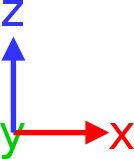
\includegraphics[width=0.04\textwidth]{DataDump/Images/Axes.png}};
			%%%%%
			\node[anchor=south west,inner sep=0] (fig_Steps0) at ({(\textwidth-\textwidth/10)*0.00+\textwidth/20},0){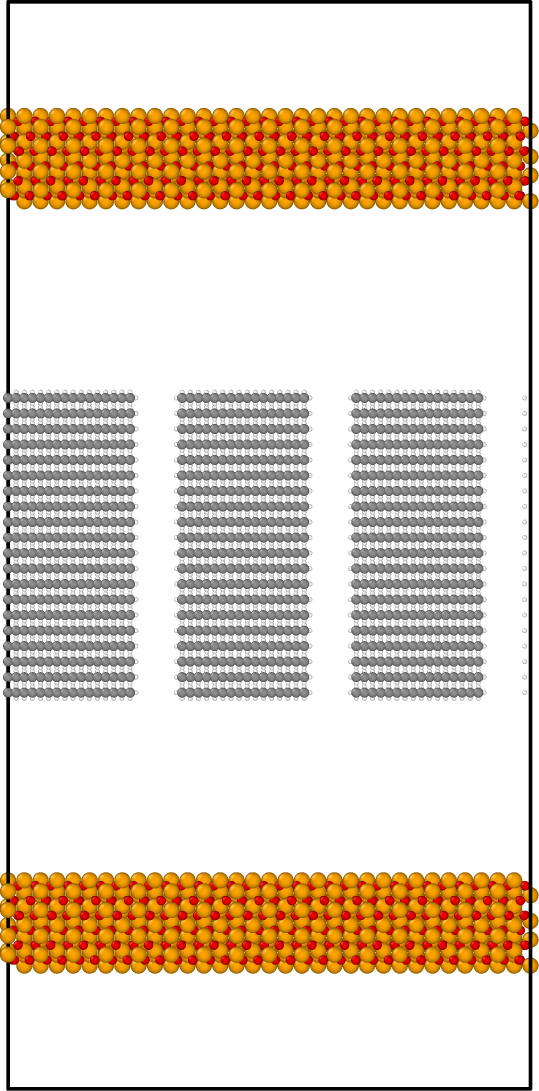
\includegraphics[width=0.150\textwidth]{DataDump/Images/1_initial.png}};
    			\support{3}{{(\textwidth-\textwidth/10)*0.00+\textwidth/20+\textwidth/24},					\textwidth/31};
    			\support{3}{{(\textwidth-\textwidth/10)*0.00+\textwidth/20+\textwidth/24+0.0669*\textwidth},	\textwidth/31};
    			\support{3}{{(\textwidth-\textwidth/10)*0.00+\textwidth/20+\textwidth/24},					0.278\textwidth}[180];
    			\support{3}{{(\textwidth-\textwidth/10)*0.00+\textwidth/20+\textwidth/24+0.0669*\textwidth},	0.278\textwidth}[180];
			%%%%%
			\node[anchor=south west,inner sep=0] (fig_Steps1) at ({(\textwidth-\textwidth/10)*0.25+\textwidth/20},0){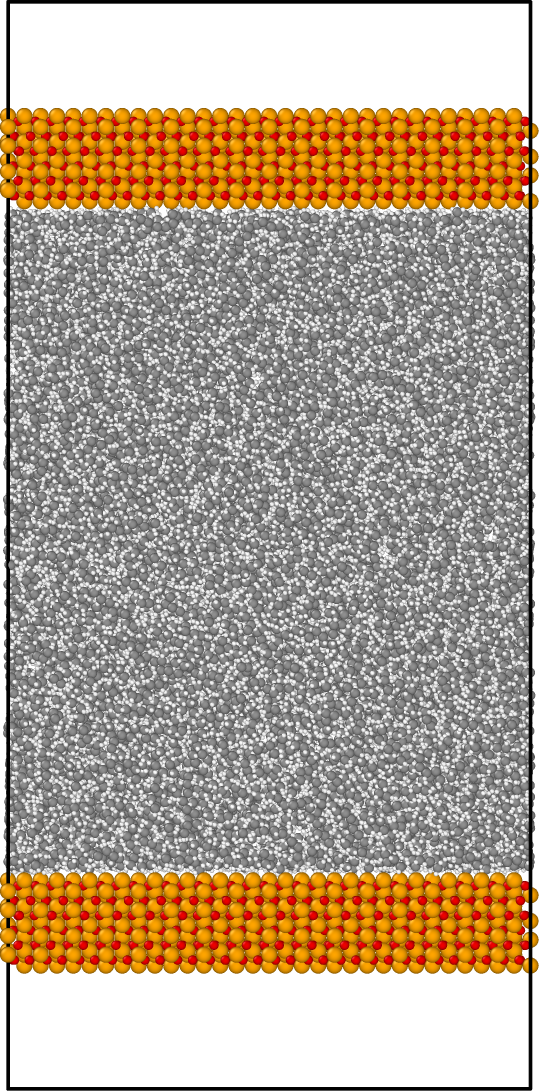
\includegraphics[width=0.150\textwidth]{DataDump/Images/2_equilibration.png}};
    			\support{3}{{(\textwidth-\textwidth/10)*0.25+\textwidth/20+\textwidth/24},					\textwidth/31};
    			\support{3}{{(\textwidth-\textwidth/10)*0.25+\textwidth/20+\textwidth/24+0.0669*\textwidth},	\textwidth/31};
    			\support{3}{{(\textwidth-\textwidth/10)*0.25+\textwidth/20+\textwidth/24},					0.278\textwidth}[180];
    			\support{3}{{(\textwidth-\textwidth/10)*0.25+\textwidth/20+\textwidth/24+0.0669*\textwidth},	0.278\textwidth}[180];
			%%%%%
			\node[anchor=south west,inner sep=0] (fig_Steps2) at ({(\textwidth-\textwidth/10)*0.50+\textwidth/20},0){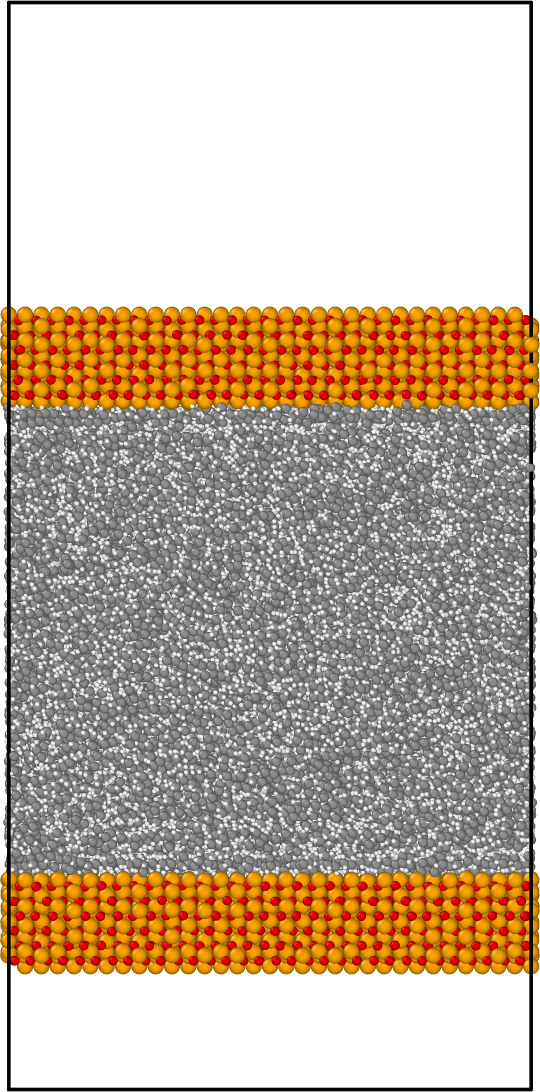
\includegraphics[width=0.150\textwidth]{DataDump/Images/3_Compression.png}};
    			\support{3}{{(\textwidth-\textwidth/10)*0.50+\textwidth/20+\textwidth/24},						\textwidth/31};
    			\support{3}{{(\textwidth-\textwidth/10)*0.50+\textwidth/20+\textwidth/24+0.0669*\textwidth},		\textwidth/31};
			\lineload{1}	{{(\textwidth-\textwidth/10)*0.50+\textwidth/20+\textwidth/110},					0.21*\textwidth}
						{{(\textwidth-\textwidth/10)*0.50+\textwidth/20+\textwidth/110+0.0669*2*\textwidth},	0.21*\textwidth}[0.5][0.5][0.11];
			\notation{5}{{(\textwidth-\textwidth/10)*0.50+\textwidth/20+\textwidth/110},					0.21*\textwidth}
						{{(\textwidth-\textwidth/10)*0.50+\textwidth/20+\textwidth/110+0.0669*2*\textwidth},	0.21*\textwidth}[$P$][][above left=0.077\linewidth];

			%%%%%
			\node[anchor=south west,inner sep=0] (fig_Steps3) at ({(\textwidth-\textwidth/10)*0.75+\textwidth/20},0){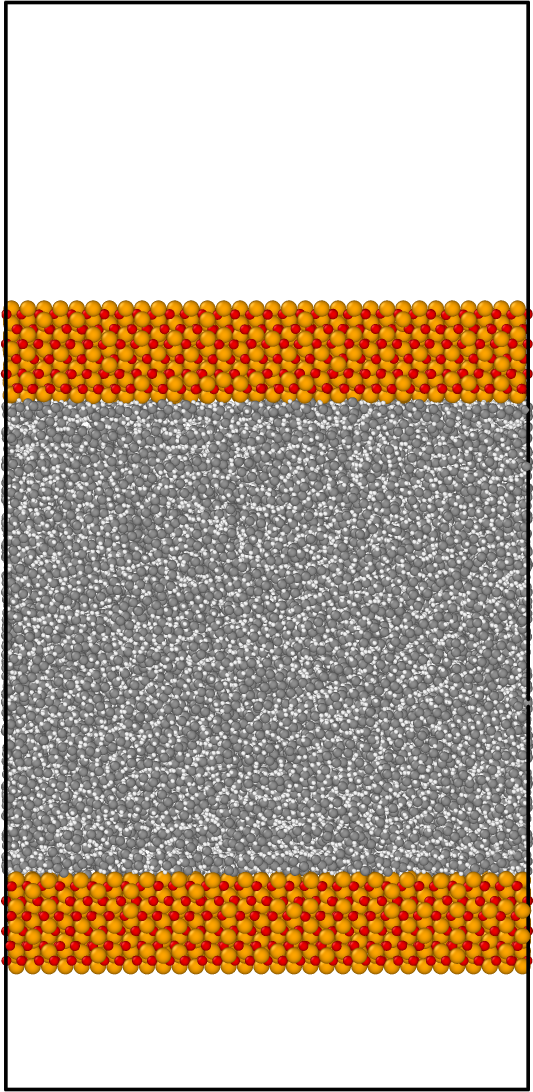
\includegraphics[width=0.148\textwidth]{DataDump/Images/4_shear.png}};
    			\support{4}{{(\textwidth-\textwidth/10)*0.75+\textwidth/20+\textwidth/24},						\textwidth/31};
    			\support{4}{{(\textwidth-\textwidth/10)*0.75+\textwidth/20+\textwidth/24+0.0669*\textwidth},		\textwidth/31};
			\lineload{1}	{{(\textwidth-\textwidth/10)*0.75+\textwidth/20+\textwidth/110},					0.21*\textwidth}
						{{(\textwidth-\textwidth/10)*0.75+\textwidth/20+\textwidth/110+0.0669*2*\textwidth},	0.21*\textwidth}[0.5][0.5][0.11];
			\notation{5}{{(\textwidth-\textwidth/10)*0.75+\textwidth/20+\textwidth/110},					0.21*\textwidth}
						{{(\textwidth-\textwidth/10)*0.75+\textwidth/20+\textwidth/110+0.0669*2*\textwidth},	0.21*\textwidth}[$P$][][above left=0.077\linewidth];
		
			\node (I) at (0.83*\textwidth, 0.206*\textwidth) {$\frac{v}{2}$} ;
			\node (J) at (0.78*\textwidth, 0.206*\textwidth) {} ;
			\draw [<- , line width=0.006*\textwidth] (I) -- (J);

			\node (K) at (0.78*\textwidth, 0.0455*\textwidth) {$\frac{v}{2}$} ;
			\node (L) at (0.83*\textwidth, 0.0455*\textwidth) {} ;
			\draw [<- , line width=0.006*\textwidth] (K) -- (L);
			

			\filldraw[fill=SERorange, draw=black] 	(0,4.5) circle (0.6125*3/4) node {Fe};
			\filldraw[fill=SERred, draw=black]  		(0,3.5) circle (0.365*3/4) node {O};
			\filldraw[fill=SERgray, draw=black]  		(0,2.5) circle (0.385*3/4) node {C};
			\filldraw[fill=SERwhite, draw=black]  	(0,1.5) circle (0.185) node {H};


			\begin{scope}[x={(fig_Steps0.south east)},y={(fig_Steps0.north west)}]
				\draw [](0.12\textwidth,-0.05) node[]{a)}	;
				\draw [](0.12\textwidth+0.225\textwidth,-0.05) node[]{b)}	;
				\draw [](0.12\textwidth+0.45\textwidth,-0.05) node[]{c)}	;
				\draw [](0.12\textwidth+0.675\textwidth,-0.05) node[]{d)}	;

			\end{scope}
		\end{tikzpicture}

		\caption{General steps carried out for the preparation and NEMD simulation of each of the the systems considered in the present work. The orange atoms represent iron (Fe), the red ones oxygen (O), the gray ones carbon (C), and the white ones hydrogen (H). a) System generation. b) Equilibration. c) Compression. d) Shear. }
		\label{fig:Steps}
	\end{center}
\end{figure*}

\pgfmathsetmacro{\SERFigwidth}{.035\linewidth}
\pgfmathsetmacro{\SERFigheight}{.026\linewidth}
\begin{figure}[htp]
    	\begin{center}
		\begin{gnuplot}[terminal=epslatex, terminaloptions={size \SERFigwidth cm, \SERFigheight cm color solid}]
			set multiplot
			#set format x  '$10^{%L}$' 
			set format y  '$10^{%L}$' 
			#set format x  '%3.1e' 
			#set format y  '%3.1e' 
			set key top left
			set xlabel "Time [\\SI{}{\\nano\\second}]"  
			set ylabel "$\\left< R^2 \\right>  [\\SI{}{\\square\\angstrom}]$"
			set logscale x
			set logscale y
			set key noautotitle
			  plot  [1e-2:1e1] [:1e5]	'DataDump/Equilibration/C16/e2e2.plot' u ($1/1e6):($2) title 'C16' ,\
						'DataDump/Equilibration/C30/e2e2.plot' u ($1/1e6):($2)  title 'C30' ,\
						'DataDump/Equilibration/C60/e2e2.plot' u ($1/1e6):($2)  title 'C60'

			set origin 0.4,0.55
			set size 0.54,0.4
			unset xlabel
			unset ylabel
			set xtics(10, 15, 20)
			#set xtics ('$10^1$' 1e1,  '$1.5\mkern-5mu\times\mkern-5mu 10^1$' 1.5e1, '$2\mkern-5mu\times\mkern-5mu 10^1$' 2e1)
			set ytics font ',80'
			plot [1e1:2e1][]	'DataDump/Equilibration/C16/e2e2.plot' u ($1/1e6):($2) ,\
							'DataDump/Equilibration/C30/e2e2.plot' u ($1/1e6):($2) ,\
							'DataDump/Equilibration/C60/e2e2.plot' u ($1/1e6):($2) 
			unset multiplot
		\end{gnuplot}
		\caption{Evolution of the mean square end-to-end distance $\left(\left< R^2 \right>\right)$ during the equilibration stage for the three considered alkane lengths: C16, C30 and C60. The main plot shows the initial equilibration at  \SI{2000}{\kelvin}; the inset the continuation at \SI{353}{\kelvin}.}
		\label{fig:e2e2}
	\end{center}
 \end{figure}

\pgfmathsetmacro{\SERFigwidth}{.035\linewidth}
\pgfmathsetmacro{\SERFigheight}{.026\linewidth}
\begin{figure}[htp]
    	\begin{center}
		\begin{gnuplot}[terminal=epslatex, terminaloptions={size \SERFigwidth cm, \SERFigheight cm color solid}]
			set multiplot
			#set format x  '$10^{%L}$' 
			set format y  '$10^{%L}$' 
			set key top left
			set xlabel "Time [\\SI{}{\\nano\\second}]"  
			set ylabel "$\\left< S^2 \\right>  [\\SI{}{\\square\\angstrom}]$"
			set logscale x
			set logscale y
			set key noautotitle
			plot   [1e-2:1e1] [:1e4]	'DataDump/Equilibration/C16/Rg2.plot'  u ($1/1e6):($2) title 'C16' ,\
						'DataDump/Equilibration/C30/Rg2.plot'  u ($1/1e6):($2) title 'C30' ,\
						'DataDump/Equilibration/C60/Rg2.plot'  u ($1/1e6):($2) title 'C60'
			set origin 0.4,0.55
			set size 0.54,0.4
			unset xlabel
			unset ylabel
			set xtics(10, 15, 20)
			#set xtics ('$10^7$' 1e7,  '$1.5\mkern-5mu\times\mkern-5mu 10^7$' 1.5e7, '$2\mkern-5mu\times\mkern-5mu 10^7$' 2e7)
			set ytics font ',80'
			plot [1e1:2e1][]	'DataDump/Equilibration/C16/Rg2.plot' u ($1/1e6):($2) ,\
							'DataDump/Equilibration/C30/Rg2.plot' u ($1/1e6):($2) ,\
							'DataDump/Equilibration/C60/Rg2.plot' u ($1/1e6):($2) 
			unset multiplot
		\end{gnuplot}
		\caption{Evolution of the mean square radius of gyration $\left(\left< S^2 \right>\right)$  during the equilibration stage for the three considered alkane lengths: C16, C30 and C60. The main plot shows the initial equilibration at \SI{2000}{\kelvin}; the inset the continuation at  \SI{353}{\kelvin}.}
		\label{fig:rg2}
	\end{center}
 \end{figure}

The last criterion, is based on the fact that systems of long chain alkanes that are not properly equilibrated can present deformation on short length scales, and this deformation is only relaxed after the chains have moved at least their own size~\cite{Auhl2003}. In order to verify this, the mean squared displacement (MSD) for the individual atoms $\left(\text{MSD}_{\text{atom}}\right)$ and for the centre of mass of the n-alkane chains $\left(\text{MSD}_{\text{CG}}\right)$ were followed during equilibration. 

Figure \ref{fig:msd} shows the $\text{MSD}_{\text{atom}}$ and $\text{MSD}_{\text{CG}}$ for the three different systems. The main plot is dedicated to the evolution at \SI{2000}{\kelvin}, with the inset showing the evolution at \SI{353}{\kelvin}. Note that due to the artificial way that the chains are first introduced into the system (see Figure \ref{fig:Steps}), the diffusivity of the longer chains is initially higher than that of the shorter chains.  If we take the length of a $C_{60}$ chain to be $\approx$ \SI{74}{\angstrom} (the angle between the C-C bonds is \SI{109.5}{\degree} and the C-C distance equal to \SI{1.54}{\angstrom}),  it can be seen that the chains move their own size after $\approx$ \SI{3e6}{} to \SI{4e6}{} steps (\SI{3}{\nano\second} to \SI{4}{\nano\second}). Taking a conservative approach, the systems are equilibrated for \SI{1e7}{} steps (\SI{10}{\nano\second}). The insets show the evolution after the temperature has been decreased; here, as expected, the slope of the $\text{MSD}_{\text{atom}}$ and $\text{MSD}_{\text{CG}}$ curves is shallower than at higher temperatures.

\pgfmathsetmacro{\SERFigwidth}{.035\linewidth}
\pgfmathsetmacro{\SERFigheight}{.026\linewidth}
\begin{figure}[htp]
    	\begin{center}
		\begin{gnuplot}[terminal=epslatex, terminaloptions={size \SERFigwidth cm, \SERFigheight cm color solid}]
			set multiplot
			#set format x  '$10^{%L}$' #'10^{%L}'
			set format y  '$10^{%L}$' #'10^{%L}'
			set xlabel "Time [\\SI{}{\\nano\\second}]"  
			set ylabel "$\\text{MSD}  [\\SI{}{\\square\\angstrom}]$"
			set key at 1.0e1, 1e3
			set logscale x
			set logscale y
			set key noautotitle
			plot [1e-2:1e1][1e2:] 	'DataDump/Equilibration/C16/msd.plot' 	 u ($1/1e6):($2) lc 1 pt 4 title 'C16',\
			   			'DataDump/Equilibration/C30/msd.plot' 			 u ($1/1e6):($2) lc 2 pt 4 title 'C30',\
			   			'DataDump/Equilibration/C60/msd.plot' 			 u ($1/1e6):($2) lc 3 pt 4 title 'C60'
			set origin 0,0
			set size 1,1

			set key at 1.5e1, 1e3
			plot [1e-2:1e1][1e2:]	'DataDump/Equilibration/C16/msd_cg.plot'  u ($1/1e6):($2)  lc 1 pt 7 title '  ',\
			   			'DataDump/Equilibration/C30/msd_cg.plot' 		  u ($1/1e6):($2)  lc 2 pt 7 title '  ',\
			   			'DataDump/Equilibration/C60/msd_cg.plot' 		  u ($1/1e6):($2)  lc 3 pt 7 title '  '

			set origin 0.145,0.55
			set size 0.54,0.4
			unset xlabel
			unset ylabel
			set xtics(10, 15, 20)
			#set xtics ('$10^7$' 1e7,  '$1.5\mkern-5mu\times\mkern-5mu 10^7$' 1.5e7, '$2\mkern-5mu\times\mkern-5mu 10^7$' 2e7)
			set ytics font ',80'
			plot [1e1:2e1][]	'DataDump/Equilibration/C16/msd.plot'  u ($1/1e6):($2) every 50 lc 1 pt 4 ,\
							'DataDump/Equilibration/C30/msd.plot'  u ($1/1e6):($2) every 50  lc 2 pt 4,\
							'DataDump/Equilibration/C60/msd.plot'  u ($1/1e6):($2) every 50  lc 3 pt 4,\
							'DataDump/Equilibration/C16/msd_cg.plot'  u ($1/1e6):($2) every 50  lc 1 pt 7,\
							'DataDump/Equilibration/C30/msd_cg.plot'  u ($1/1e6):($2) every 50  lc 2 pt 7,\
							'DataDump/Equilibration/C60/msd_cg.plot'  u ($1/1e6):($2) every 50  lc 3 pt 7


			unset multiplot
		\end{gnuplot}
		\caption{Evolution of the mean squared displacement (MSD) during the equilibration stage for the three considered alkane lengths: C16, C30 and C60. The main plot shows the initial equilibration at  \SI{2000}{\kelvin}; the inset the continuation at  \SI{353}{\kelvin}. The full circles represent the mean squared displacement per atom $\left(\text{MSD}_{\text{atom}}\right)$ while the empty squares the mean squared displacement per centre of mass of chain $\left(\text{MSD}_{\text{CG}}\right)$.}
		\label{fig:msd}
	\end{center}
 \end{figure}

\section{Transient Velocity Profiles}

A representative example of transient deviations from Couette flow at the onset of shear is shown for $C_{30}$, \SI{1.0}{\giga\pascal} and  \SI{50}{\meter\per\second} in Figure \ref{fig:VelProf_MDP}. Most systems eventually show Couette flow, but non-linear flow persists into the steady state for some of the systems and conditions studied (Figure \ref{fig:VelProf_MDP2}).

\pgfmathsetmacro{\SERFigwidth}{.035\linewidth}
\pgfmathsetmacro{\SERFigheight}{.026\linewidth}
\begin{figure}[htp]
    	\begin{center}
		\begin{gnuplot}[terminal=epslatex, terminaloptions={size \SERFigwidth cm, \SERFigheight cm color solid}]

			set key bottom right
			set xlabel "z coordinate"  
			set ylabel "x Velocity $\\left[ \\SI{}{\\meter\\per\\second} \\right]$"
			set xrange [-50:50]
			set yrange [-30:30]
			set ytics -40,20,40
			plot  	'DataDump/Shear/C30/1.0GPa/50m_s/vel_prof_x_s_40.dump' u ($2-37.01):($4*100) w l  lt 7 lw 2  title               "$\\SI{0.4}{\\nano\\second}$",\
					'DataDump/Shear/C30/1.0GPa/50m_s/vel_prof_x_s_200.dump' u ($2-37.77):($4*100) w l  lt 8 lw 2  title     "$\\SI{2}{\\nano\\second}$",\
					'DataDump/Shear/C30/1.0GPa/50m_s/vel_prof_x_s_500.dump' u ($2-37.52):($4*100) w l  lt 9 lw 2  title     "$\\SI{5}{\\nano\\second}$"
					
		\end{gnuplot}
		\caption{Velocity profiles along x at three different times during the transient state of the simulation. Results are presented for the case of  C30,  \SI{1.0}{\giga\pascal} and  \SI{50}{\meter\per\second}.}
		\label{fig:VelProf_MDP}
	\end{center}
 \end{figure}

\end{document}

%%%%%%%%%%%%%%%%%%%%%%%%%%%%%%%%%%%%%%%%%%%%%%%%%
%%%%%%%%%%%%%%%%%%%%%%%%%%%%%%%%%%%%%%%%%%%%%%%%%
%%%%%%%%%%%%%%%%%%%%%%%%%%%%%%%%%%%%%%%%%%%%%%%%%

%git pull
%git add -A
%git commit
%git push origin master


